In the following sections, our experiments are defined and have their results reported and analysed.
We go over the minutia of the algorithmic details and the software and hardware resources employed in the conducted experiments, and afterward, we discuss how the proposed solution from Chapter ~\ref{ch:methodology} fared in this scenario.


\section{Experiments Definition}\label{sec:experiments-definition}

The proposed methodology was implemented in the R language version 4.0.2 (2020-06-22), and the main libraries used were \textit{caret}, \textit{recipes}, and others from the \textit{tidyverse} and \textit{tidymodels} collections.
Max Kuhn's \textit{caret} (Classification And REgression Training) is a feature-rich machine learning framework~\cite{Kuhn2008}, which was crucial for the implementation of the model induction and evaluation pipeline, along with \textit{recipes} and \textit{rsample} that were leveraged for preprocessing, and resampling respectively.

On the data manipulation side, the main libraries used were \textit{tibble} (for in-memory data model), \textit{reader} (for data ingestion), \textit{dplyr} and \textit{tidyr} (for general tibble processing), \textit{purrr} (for functional programming support), and \textit{ggplot2} (for visualization), all part of the \textit{tidyverse} collection.

As for the main supervised learning algorithms, we chose to run our experiments with three methods.
Elastic net logistic regressions were selected so that we have linear models with good odds of reasonable interpretability.
Additionally, as mentioned in Chapter~\ref{ch:related_work}, this algorithm was employed by~\citet{Librenza-Garcia2020} over the dataset from the ELSA-Brasil study.
The Elastic Net models were fit using the \textit{glmnet} package implementation~\cite{Friedman2010}.

Our second leaner of choice was the multilayer perceptron, as it is a generally well-performing and customizable technique and is among the most frequently used algorithms from the systematic literature review from~\citet{Burke2019}, as shown in Chapter~\ref{ch:related_work}.
Its R implementation in this study was the \textit{mlpML} from the package RSNNS (short for "an R port of the Stuttgart Neural Network Simulator")~\cite{Bergmeir2012}, which although it is not the most efficient or the fastest available is sufficiently practical for our needs - we intended to keep the architectures simple.

Finally, random forests were selected to be trained too, as they are a quite popular algorithm among medical applications of ML\@.
Also, we are interested in RFs for their potentially higher complexity compared to the other two algorithms, for being an ensemble of several trees.
Random forests, in our experiments, were induced using the \textit{ranger} package, which is efficient and apt for high dimensionality data ~\cite{Wright2017}.

Considering the afore-mentioned choices of algorithms, it would be reasonable to encode our attributes with one-hot encoding to avoid that the models infer ordinal relations in categorical data.
That said, as our dataset is vast in features, we chose to not make use of this technique, mainly because it would multiply our number of variables which is already large, and manually analyzing which features to encode to reduce this effect would be costly.

As our pipeline requires lots of parameter definitions, we provide a list of the ones used in our experiments in Table~\ref{tab:pipeline-parameters-experiments}.
Arguably the most relevant one is the final ratio of class distributions, which was chosen to be 1:1 to balance the data.
We decided to have the pipeline parameters fixed for every algorithm induction, as the opposite would be time-consuming.

\begin{table}[h]
    \caption{Pipeline parameters used in experiments}
    \begin{center}
        \begin{tabular}{l|c}
            \textit{Parameter}                             & \textit{Value}                                   \\
            \hline
            \hline
            Evaluation CV - K (folds)                      & 10                                               \\
            Evaluation CV - N (times)                      & 3                                                \\
            RFE Training CV - K (folds)                    & 5                                                \\
            RFE Training CV - N (times)                    & 2                                                \\
            Base Training CV - K (folds)                   & 5                                                \\
            Base Training CV - N (times)                   & 2                                                \\
            Downsampling - P-class ratio                   & 33.3\%                                           \\
            SMOTE - P-class ratio                          & 50\%                                             \\
            SMOTE - nearest neighbors                      & 5                                                \\
            NZV Filter - Dominant value max prevalence     & 0.95                                             \\
            NZV Filter - Unique values min frequency       & 0.1                                              \\
            Correlation Filter - Threshold                 & 0.9                                              \\
            Correlation Filter - Method                    & \textit{Pearson}                                 \\
            NA Imputation - Method                         & Mean value                                       \\
            RFE Best Attribute set sizes                   & (2^k)$^{\text{k=9}}_{\text{k=3}}$                \\
            Elastic Net GS - Alphas values                 & 0.1 , 0.325 , 0.550 , 0.775 , 1                  \\
            Elastic Net GS - Lambda values                 & 2e-4 , 9.2e-4 , 4.3e-3 , 2e-2 , 9.2e-2           \\
            Neural Network GS - Layer 1 \#Units            & 1 , 2 , 3 , 4 , 5                                \\
            Neural Network GS - Layer 2 \#Units            & 0 , 1 , 2 , 3 , 4                                \\
            Random Forest GS - Random-attributes set sizes & 2, 17, 33, 48, 64                                \\
            Random Forest GS - Node-splitting methods      & \textit{gini}, \textit{extratrees}               \\
            Weighted-Averaging Ensemble - Weights          & Equal (\sfrac{1}{3}, \sfrac{1}{3}, \sfrac{1}{3}) \\
            \hline
        \end{tabular}
    \end{center}
    \label{tab:pipeline-parameters-experiments}
\end{table}

To speed up the experiments, we used three different computers.
Each one has an equal amount of RAM (16GB), but they differ in their processors and operational systems.
The first one has a quad-core Intel Core i7-4770K CPU running in 7 threads over Arch Linux, and executed a pipeline run of \textit{ranger}, taking about 7 days to finish.
The second one runs Linux Mint Tara over an Intel Core i7-7700HQ quad-core CPU using 7 threads, which remarkably ran the procedures for \textit{glmnet} in a single day.
Finally, the third computer uses 14 threads in MacOS Catalina over an octa-core Intel Core i9-9880H and was used to train the \textit{mlpML} multilayer perceptrons for a whole week.


\section{Results Analysis}\label{sec:results-analysis}

In the following subsections, we examine our learners' characteristics by focusing our attention on three different facets.
First, Subsection~\ref{subsec:final-performance-analysis} summarizes the performances obtained by our model and reviews the proposed weighted-averaging ensemble.
Sequentially, Subsection~\ref{subsec:hyperparameters-analysis} describes the trained models in terms of their tuned hyperparameters.
Lastly, Subsection ~\ref{subsec:feature-selection-analysis} presents the characterizations of the models in terms of their decision-making criteria, exploring the most determining attributes most for the suicidality classification.

\subsection{Classification Performance Analysis}\label{subsec:final-performance-analysis}

The most critical characteristic of our models is how competent they are at solving the task of classification of suicidality.
To assess that information, we compare the elastic nets, multilayer perceptrons, random forests, and ensembles (having one of those for each final evaluation CV) with respect to their F\textsubscript{2}-Score, AUCROC, sensitivity, and specificity.
We display the mean and standard deviation measurements of these quantities in Table~\ref{tab:final-performance-estimates} (with entries ordered by F\textsubscript{2}-Score), while Figures~\ref{fig:boxplot-f2},~\ref{fig:boxplot-aucroc},~\ref{fig:boxplot-sens},~\ref{fig:boxplot-spec} graphically compare the distribution of measurements of each metric over the cross-validation resamples.

Table~\ref{tab:final-performance-estimates} shows our ensemble approach was successful in increasing the overall performance robustness.
It generally displays the best qualities of the other individual models in a single one.
The averaging mechanism has the best F\textsubscript{2}-Score and second-best sensitivity, paired with the ANNs, and the best AUCROC, together with the random forests.
It also has the second-best specificity, although the score gap between it and the winner in that regard, the forests, is significant.
In conclusion, the boxplots and the table give us two crucial take-aways.
On the one hand, our models are diverse and heterogeneous w.r.t.\ their error-type profiles.
RFs tend to be way more restrained in predicting the positive class, as opposed to MLPs, while ENs (just as we saw when analyzing attributes) show an intermediate degree in that spectrum where the others are opposites.
On the other hand, combining the three algorithms with an averaging-probability ensemble yields a performance profile considerably better than the mean of the performance of its constituents.
As will be presented in subsection~\ref{subsec:feature-selection-analysis}, the trained models also have complementary decision-making criteria, which further motivates and explains the success of the ensemble.

\begin{table}[h]
    \caption{Final performance estimates mean and standard deviation}
    \begin{center}
        \begin{tabular}{c|c|c|c|c|c|c|c|c}
            \textit{Algorithm}    & \textit{F\textsubscript{2}-Score} & \textit{AUCROC}      & \textit{Sensitivity} & \textit{Specificity} \\
            \hline
            \hline
            Ensemble              & 0.690 \textpm\ 0.029              & 0.811 \textpm\ 0.018 & 0.780 \textpm\ 0.049 & 0.666 \textpm\ 0.047 \\
            Multilayer Perceptron & 0.686 \textpm\ 0.042              & 0.764 \textpm\ 0.081 & 0.807 \textpm\ 0.093 & 0.591 \textpm\ 0.173 \\
            Elastic Net           & 0.659 \textpm\ 0.066              & 0.773 \textpm\ 0.042 & 0.747 \textpm\ 0.112 & 0.659 \textpm\ 0.095 \\
            Random Forest         & 0.608 \textpm\ 0.041              & 0.814 \textpm\ 0.019 & 0.630 \textpm\ 0.048 & 0.792 \textpm\ 0.026 \\
            \hline
        \end{tabular}
    \end{center}
    \label{tab:final-performance-estimates}
\end{table}

\begin{figure}[H]
    \caption{Comparison of measured F\textsubscript{2}-Score for different algorithms}
    \centerline{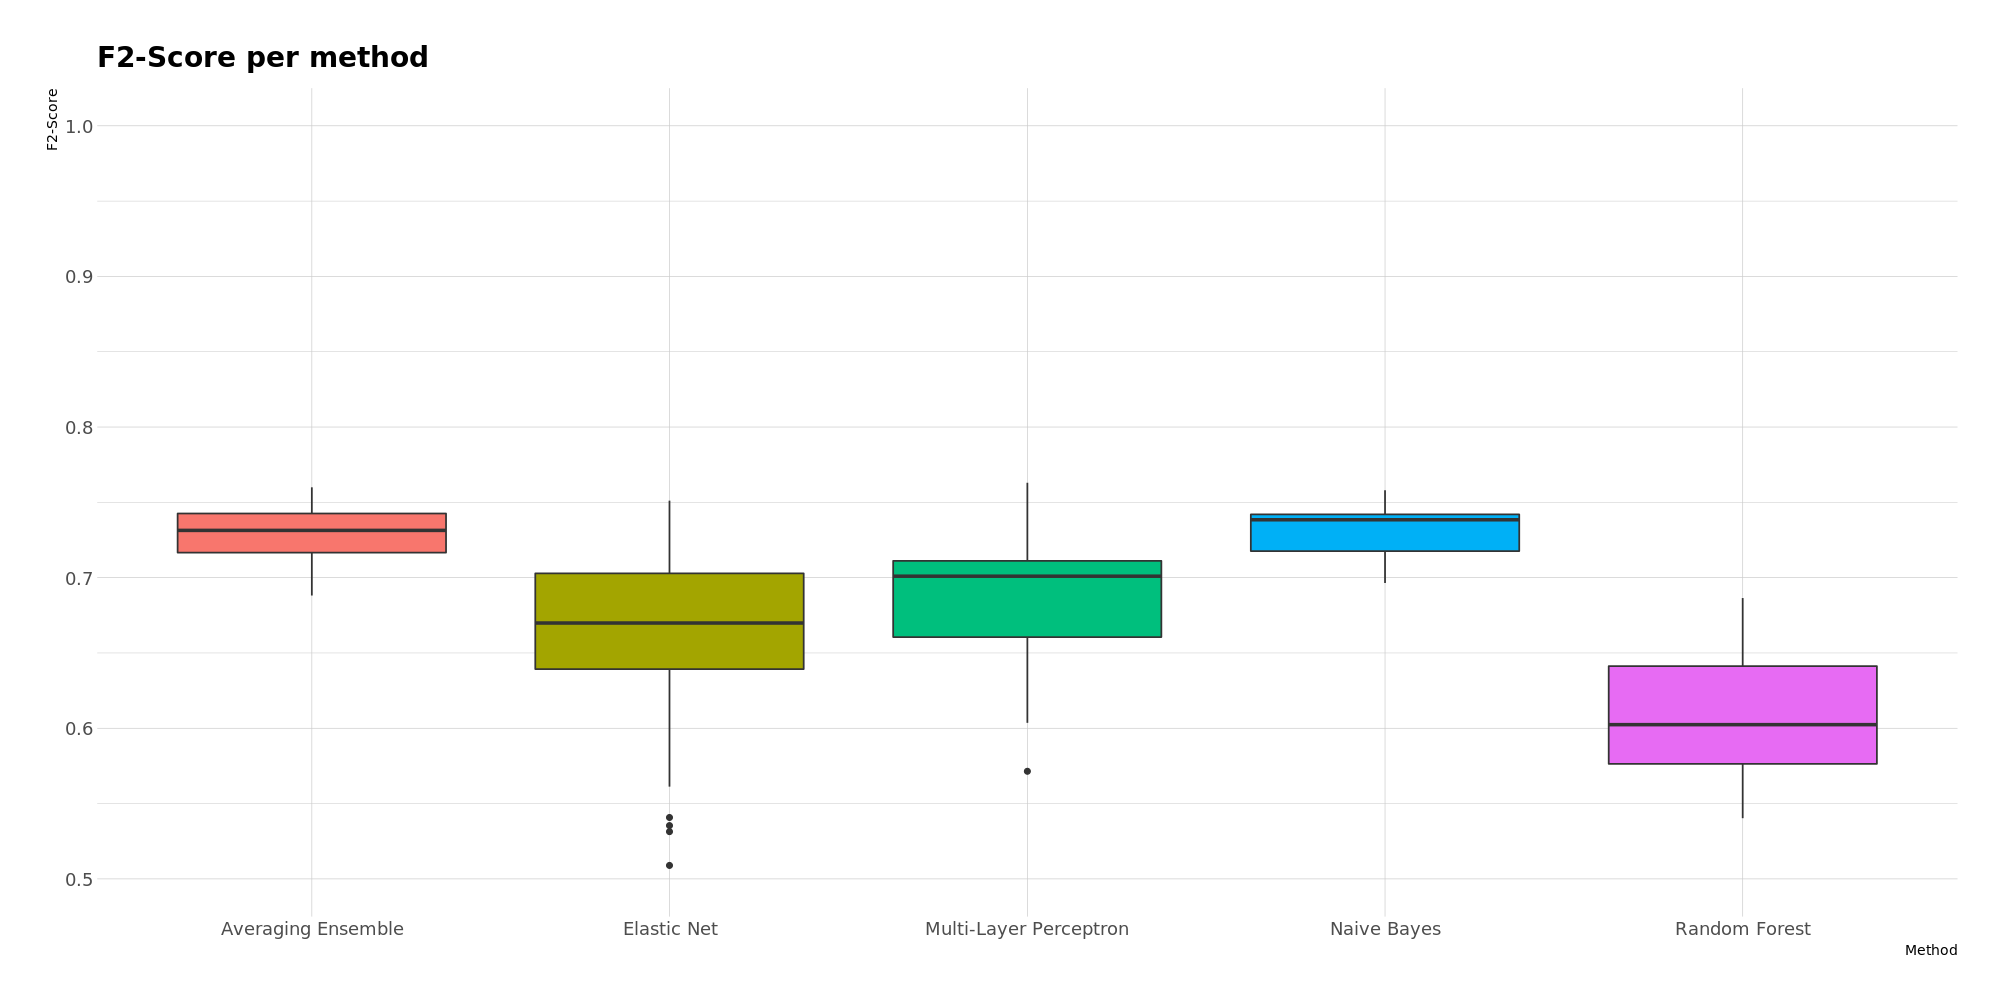
\includegraphics[scale=.2]{../reports/results/models_and_evals/summary/box_plot_f2.png}}
    \label{fig:boxplot-f2}
\end{figure}

\begin{figure}[H]
    \caption{Comparison of measured AUCROC for different algorithms}
    \centerline{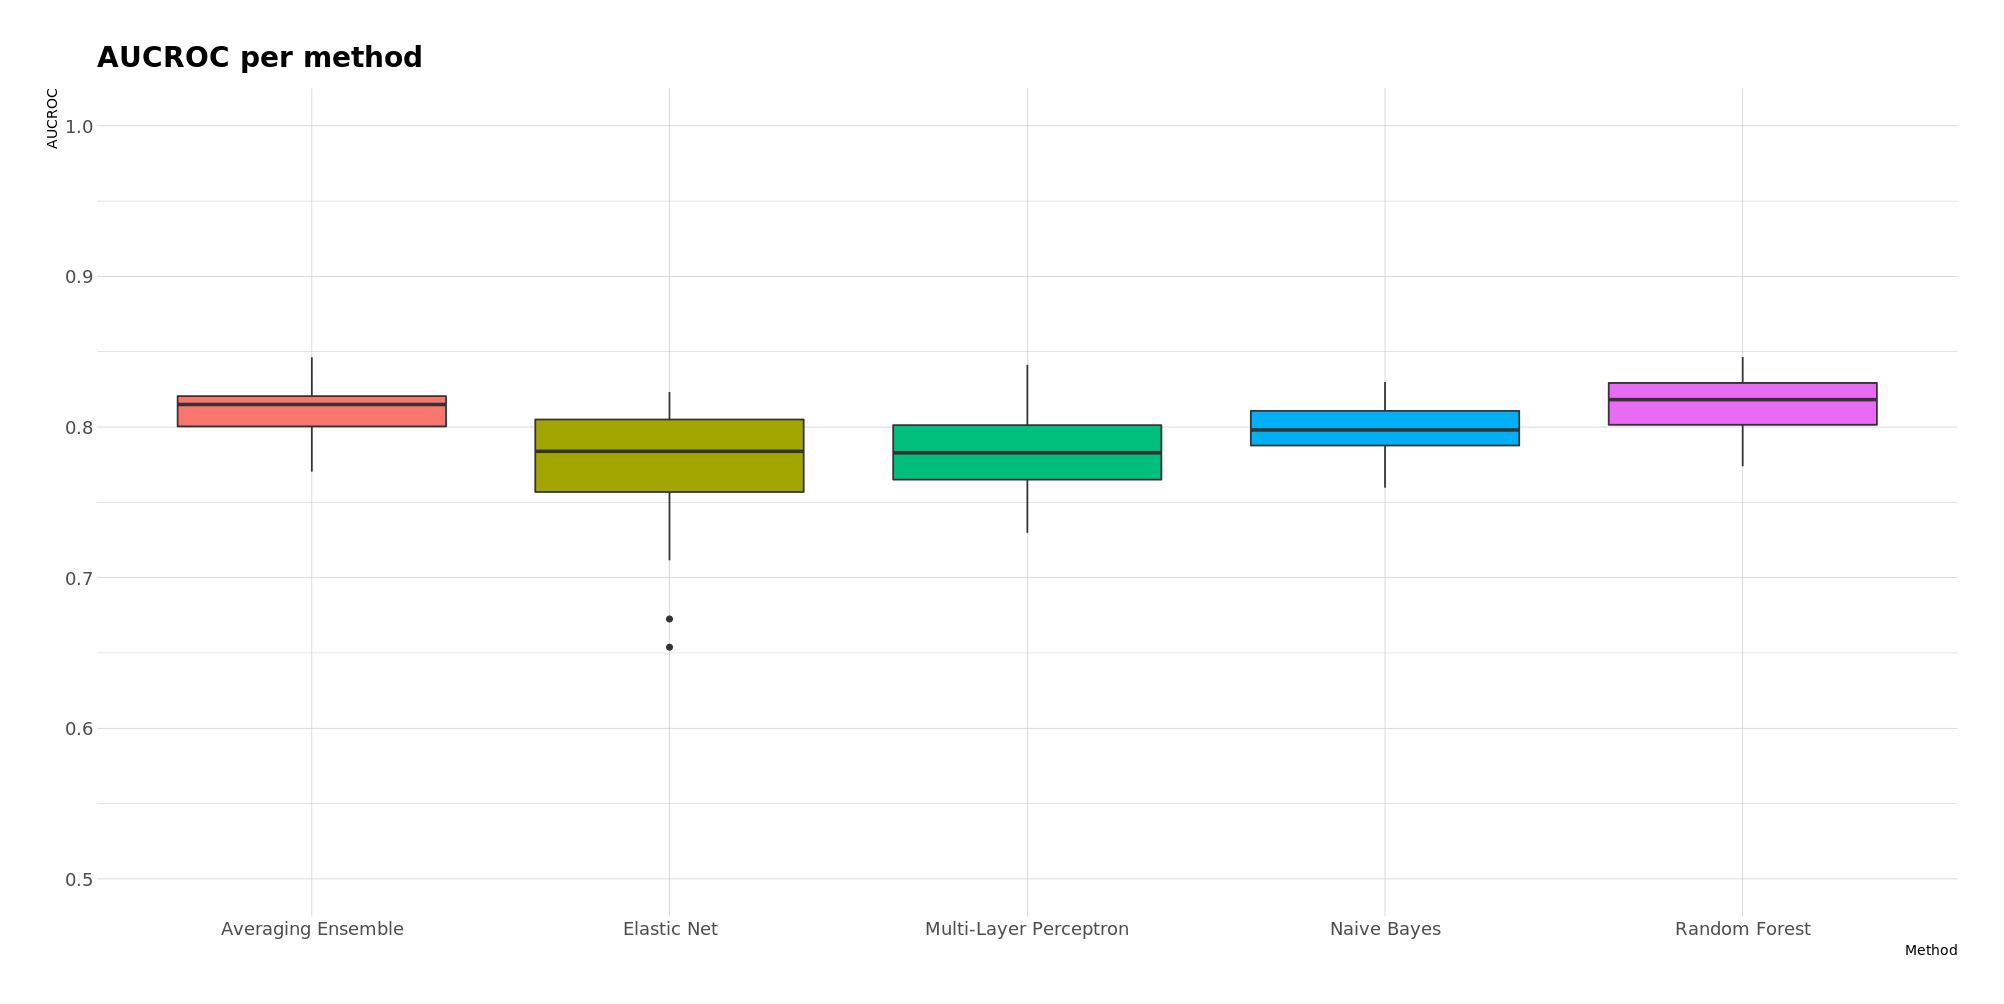
\includegraphics[scale=.2]{../reports/results/models_and_evals/summary/box_plot_aucroc.png}}
    \label{fig:boxplot-aucroc}
\end{figure}

\begin{figure}[H]
    \caption{Comparison of measured sensibility for different algorithms}
    \centerline{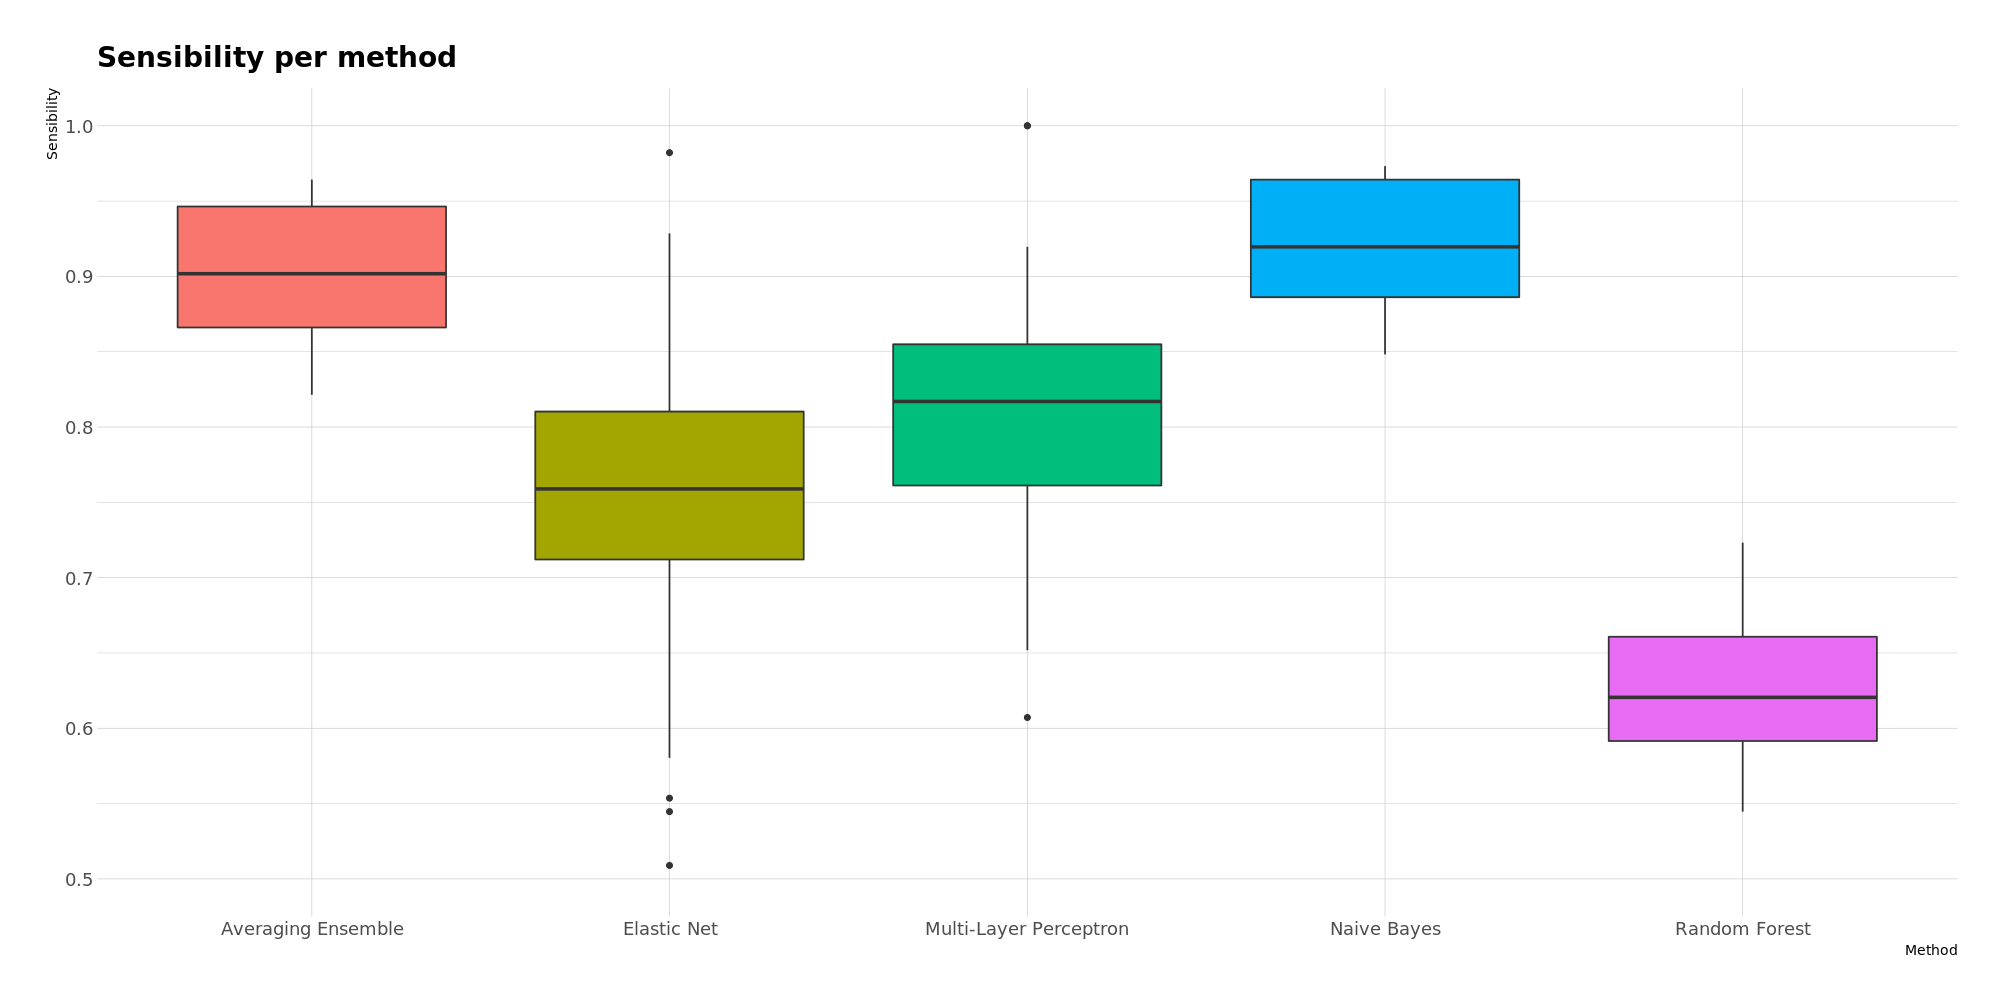
\includegraphics[scale=.2]{../reports/results/models_and_evals/summary/box_plot_sens.png}}
    \label{fig:boxplot-sens}
\end{figure}

\begin{figure}[H]
    \caption{Comparison of measured specificity for different algorithms}
    \centerline{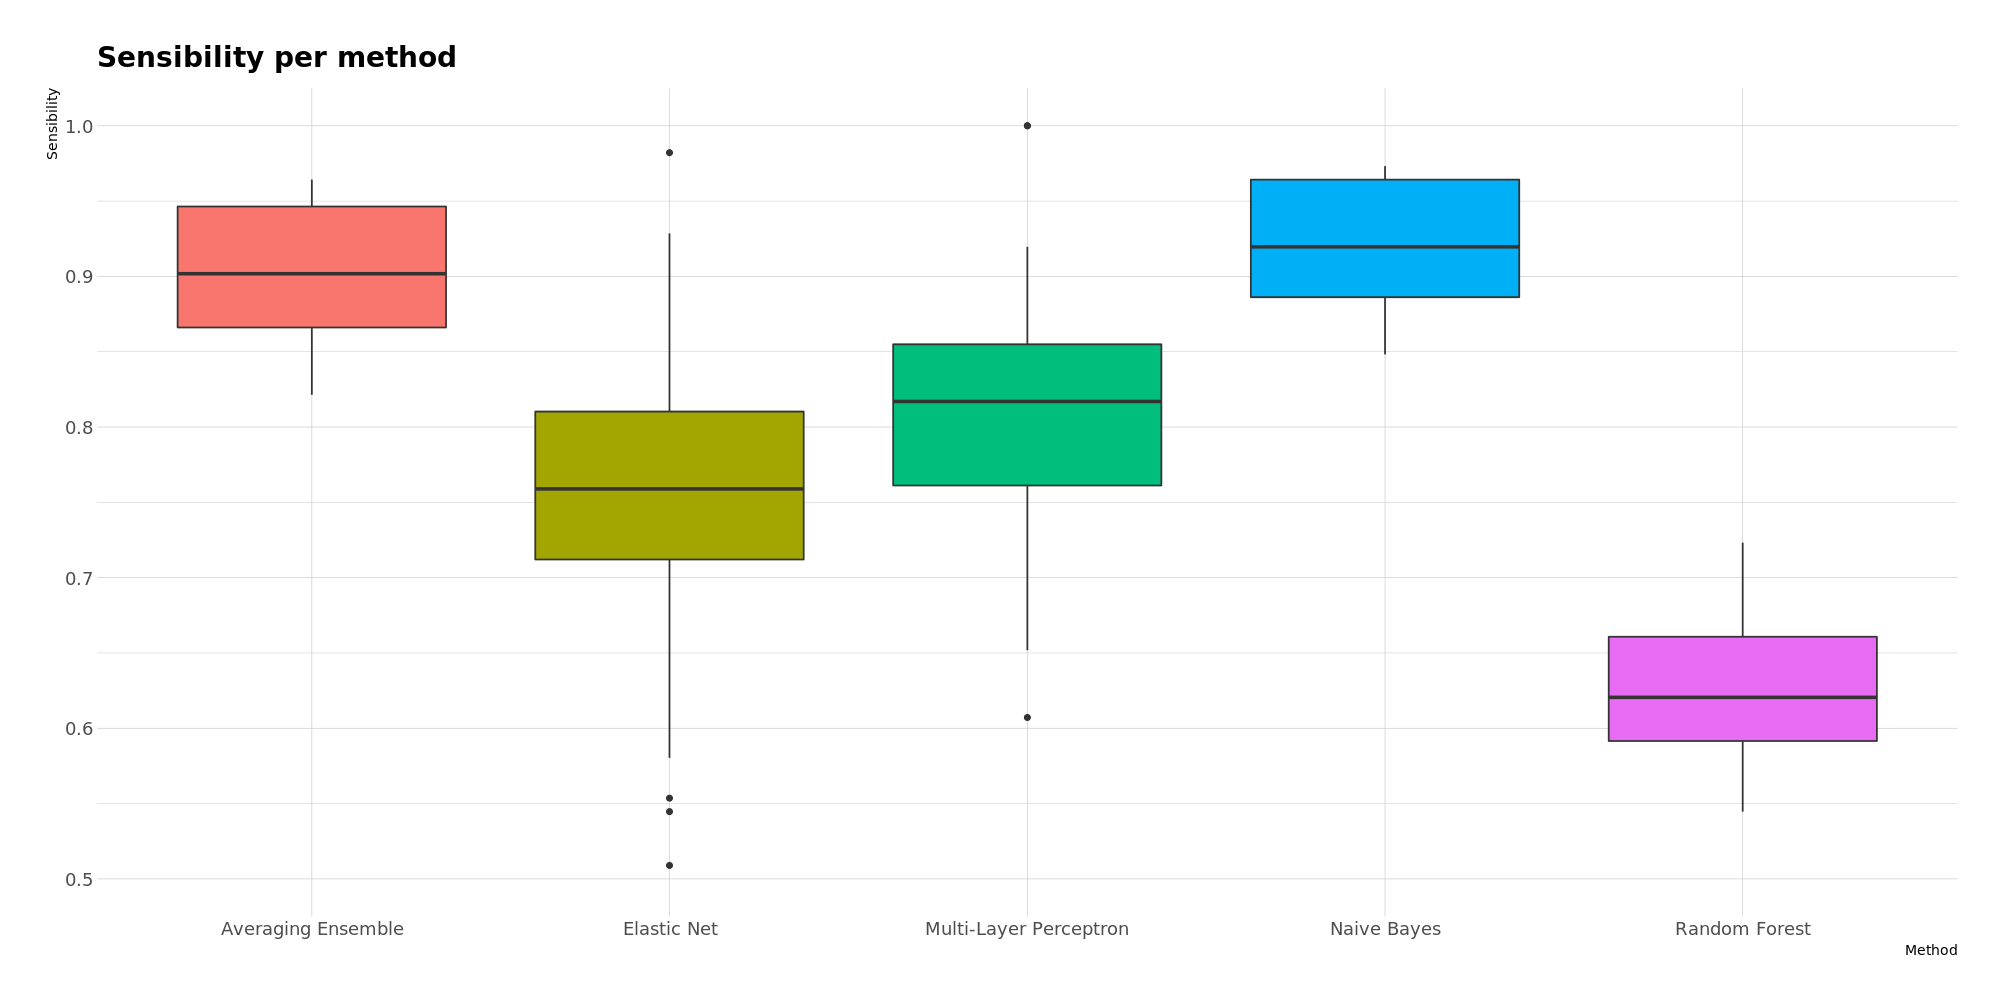
\includegraphics[scale=.2]{../reports/results/models_and_evals/summary/box_plot_spec.png}}
    \label{fig:boxplot-spec}
\end{figure}

\subsection{Hyperparameters Analysis}\label{subsec:hyperparameters-analysis}

\begin{table}[h]
    \caption{Hyperparameters most-frequently chosen in tuning}
    \begin{center}
        \begin{tabular}{l|c}
            \textit{Parameter}                    & \textit{Value}      \\
            \hline
            \hline
            Elastic Net - Alphas                  & 0.1                 \\
            Elastic Net - Lambda                  & 0.09                \\
            Neural Network - Layer 1 \#Units      & 1                   \\
            Neural Network - Layer 2 \#Units      & 1                   \\
            Random Forest - Node-splitting method & \textit{extratrees} \\
            Random Forest - \#Random-attributes   & 2                   \\
            \hline
        \end{tabular}
    \end{center}
    \label{tab:most-frequent-hyperparams}
\end{table}

For the analysis of the produced models internal characteristics, it is proper to first verify the results of the hyperparameters tuning process, as this plays an important role in models' performance.
The most frequently chosen hyperparameters values of the final models are summarized in Table~\ref{tab:most-frequent-hyperparams} and indicate that, in general, relatively simpler models tend to perform better in the training phase.
This is not surprising, since the best sizes of variables subsets are low and in the hyperparameters tuning phase the available data has a relatively small number of instances, thus it is probably the case the more complex models could overfit and perform poorly.

Figures~\ref{fig:params-ranger},~\ref{fig:params-mlp}, and ~\ref{fig:params-glmnet} show plots of the F\textsubscript{2}-Score during the training of the base-learners' model of a given resample, for multiple combinations of parameters of RFs, ANNs, and ENs (respectively).
We see that, at least for this fold (and we keep the graphical analysis limited to this single one for the sake of simplicity), performance estimates seem to vary in an orderly manner throughout the hyperparameter values planes.
More specifically, clear patterns are identifiable in every hyperparameters plot.

First, in the RF graph of Figure~\ref{fig:params-ranger}, where the \textit{extratrees} (extremely randomized trees) and the \textit{gini} tree-node-splitting methods are compared, we find that there is a big in the F\textsubscript{2}-Score between the two, but for both we observe relatively flat lines for higher values of randomly selected predictors (\textit{NRand}).
For the lower values (i.e.\ from the range between 2 and 20), with the increasing number of predictors, F\textsubscript{2}-Score increases in the \textit{gini} line, but decreases for the extremely randomized trees splitting method.
Most notably, the peak score is found in the left-most point of the \textit{extratrees} line.

\begin{figure}[H]
    \caption{Hyperparameter tuning for Random Forest in first CV resample}
    \centerline{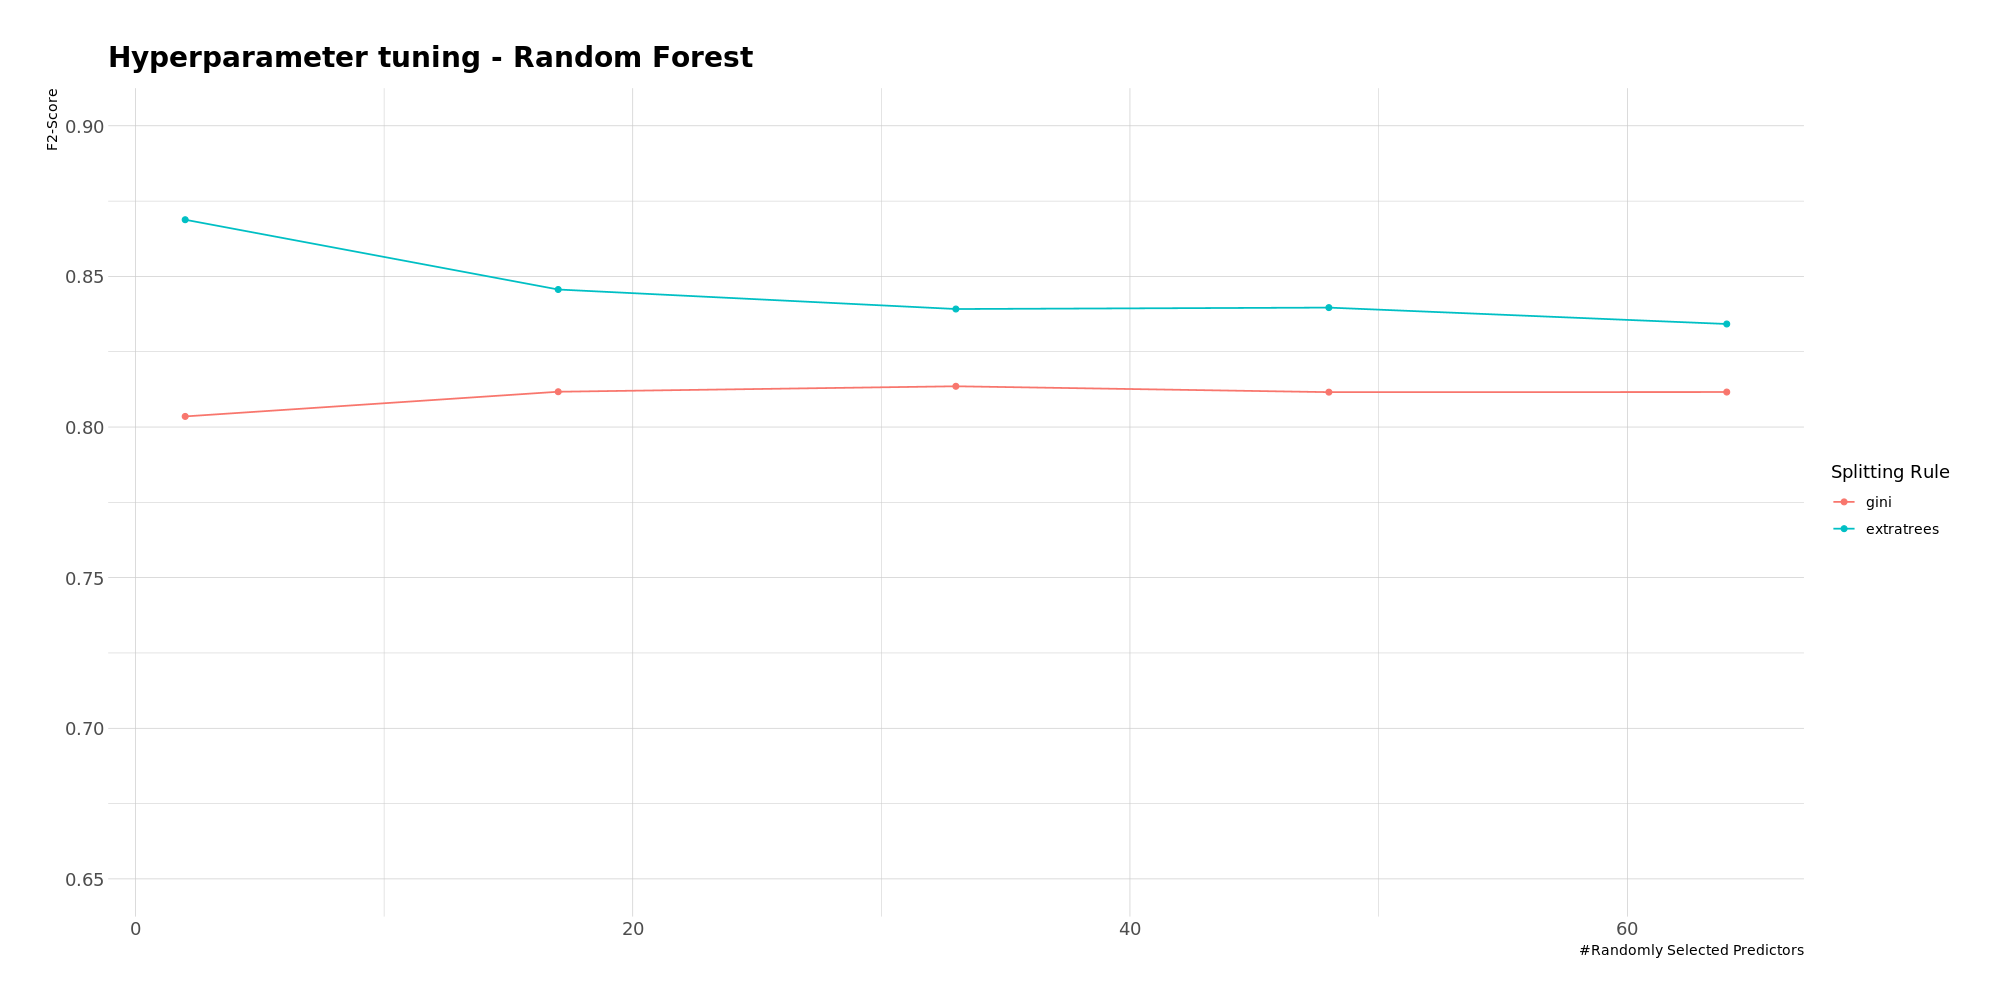
\includegraphics[scale=.21]{../reports/results/models_and_evals/summary/params_ranger_resample_1.png}}
    \label{fig:params-ranger}
\end{figure}

\begin{figure}[H]
    \caption{Hyperparameter tuning for Multilayer Perceptron in first CV resample}
    \centerline{\includegraphics[scale=.21]{../reports/results/models_and_evals/summary/params_mlpML_resample_1.png}}
    \label{fig:params-mlp}
\end{figure}

\begin{figure}[H]
    \caption{Hyperparameter tuning for Elastic Net in first CV resample}
    \centerline{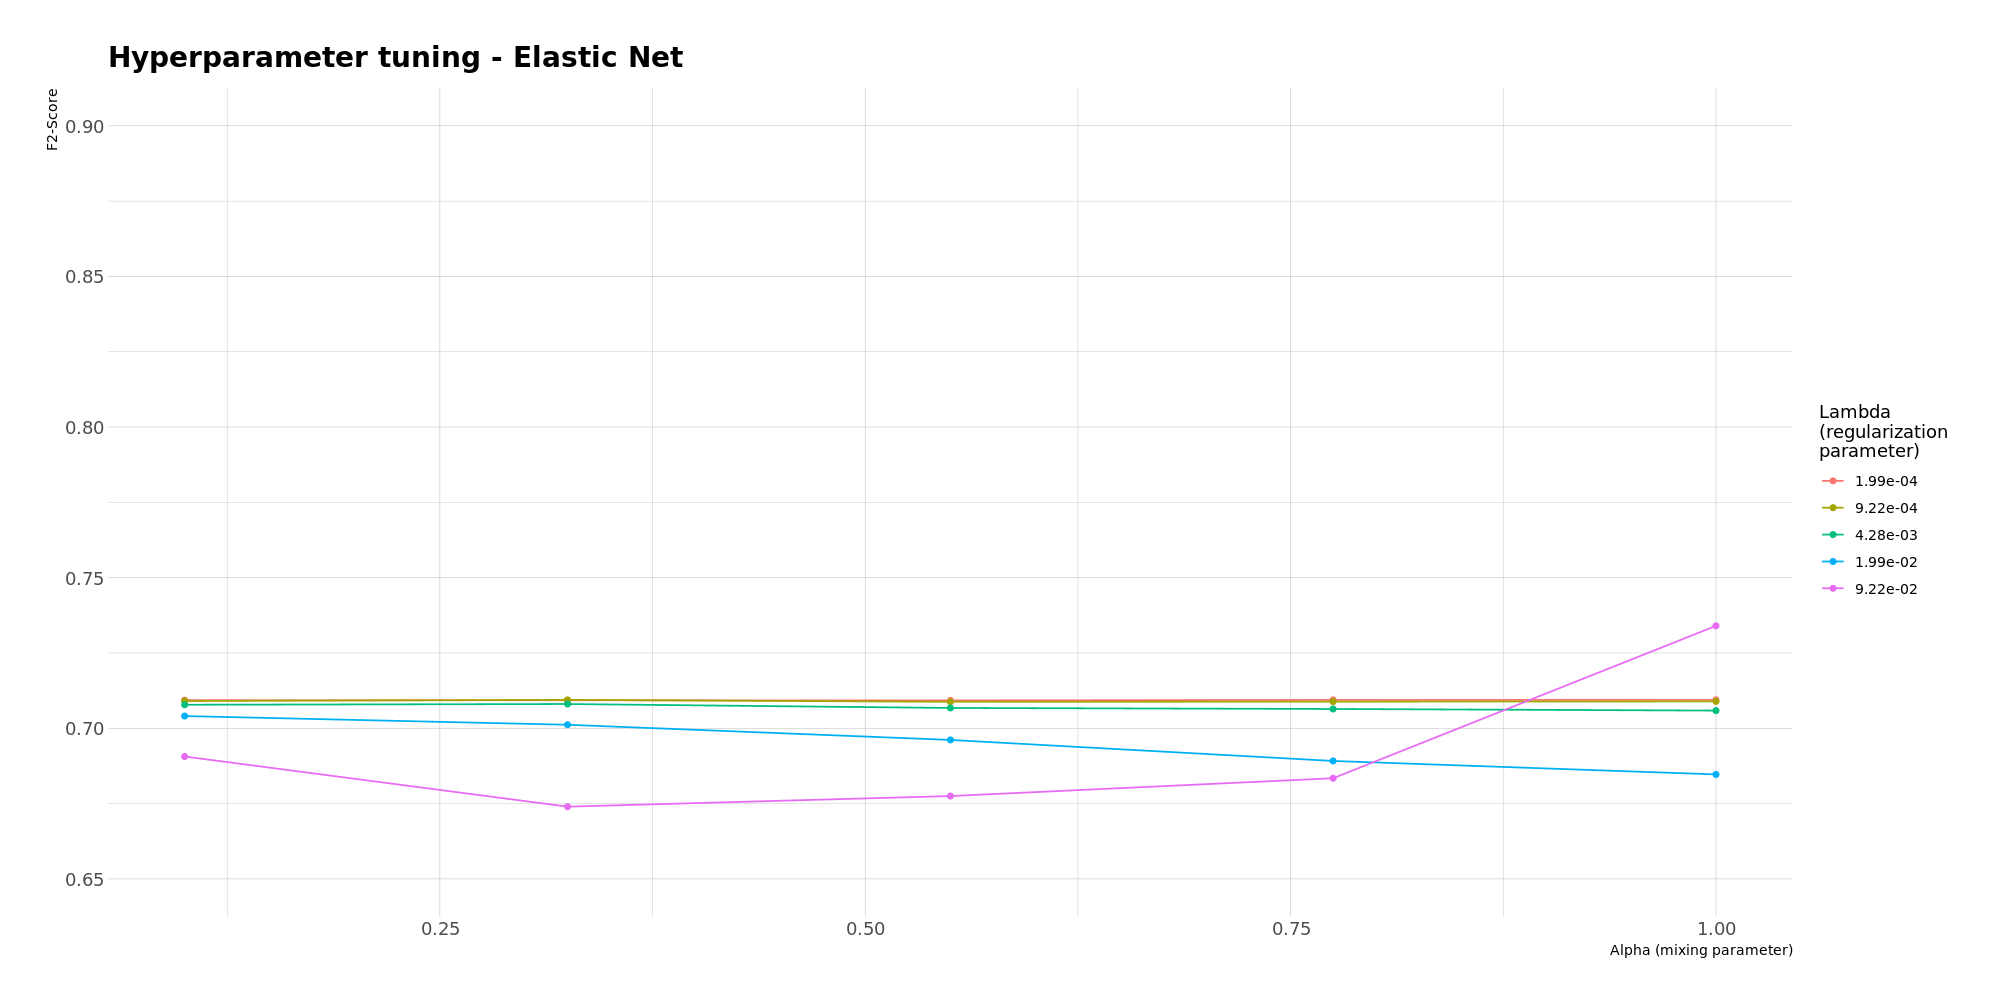
\includegraphics[scale=.21]{../reports/results/models_and_evals/summary/params_glmnet_resample_1.png}}
    \label{fig:params-glmnet}
\end{figure}

As for Figure~\ref{fig:params-mlp}, every colored line represents a neural network with a given number of neurons in the second (and last) hidden layer.
The commonalities between these slightly different architectures is that performance is lower for higher numbers of hidden units of layer 1 (although it varies in a bowl-shaped curve).
Increasing the number of neurons in layer 2 has a similar effect.
In other words, simpler ANNs, in our scenario, seem to carry out a better classification.

Lastly, the plot of EN's hyperparameters of Figure~\ref{fig:params-glmnet} indicates a similar behavior to the one seen for the random forest, in the sense that each line generally presents just small variations of F\textsubscript{2}-Score with respect to the variable from the horizontal axis (the lasso-ridge mixing parameter alpha in this case).
Also in the same manner as the RF's grid search, the maximum performance of this particular elastic net was achieved in an "extreme" value, the highest \textit{lambda} and highest \textit{alpha} pair (as it is with the lowest RF's \textit{NRand}).
This is curious to notice, as an \textit{alpha} value of 1 indicates a purely lasso regression.

\subsection{Feature Selection Analysis}\label{subsec:feature-selection-analysis}

Besides hyperparameters tuning, another characteristic worth examining is the models' predictive capabilities across different predictor sets of the RFE loops.
For each final RFE model produced, Figures~\ref{fig:rfe-glmnet},~\ref{fig:rfe-mlp}, and~\ref{fig:rfe-ranger} show the F\textsubscript{2}-Score variation depending on the number of variables considered in the base learners induction.
To analyse the algorithms' performance according to distinct features set sizes, it is useful to start the analysis of the results by the right side of the graph, which represents the original features set size.
This last mark in the horizontal axis indicates the data has as many variables as the cleansed dataset, which are then reduced in quantity down to about 600 by the base learners preprocessing.
As the RFE retrains and reassesses the variables importances at each iteration, the difference between the number of predictors before and after preprocessing should drastically diminish.
It is curious that both elastic nets (Figure ~\ref{fig:rfe-glmnet}) and ANNs (~\ref{fig:rfe-mlp}) tend to perform better with fewer variables, showing a smoothly varying F\textsubscript{2}-Score curve.
On the other hand, random forests present a performance peak at the predictor set size of 64 (Figure~\ref{fig:rfe-ranger}), which indicates that after further removal of variables, too much valuable information is taken out from the model training process.

\begin{figure}[H]
    \caption{Recursive feature elimination performance for Elastic Net}
    \centerline{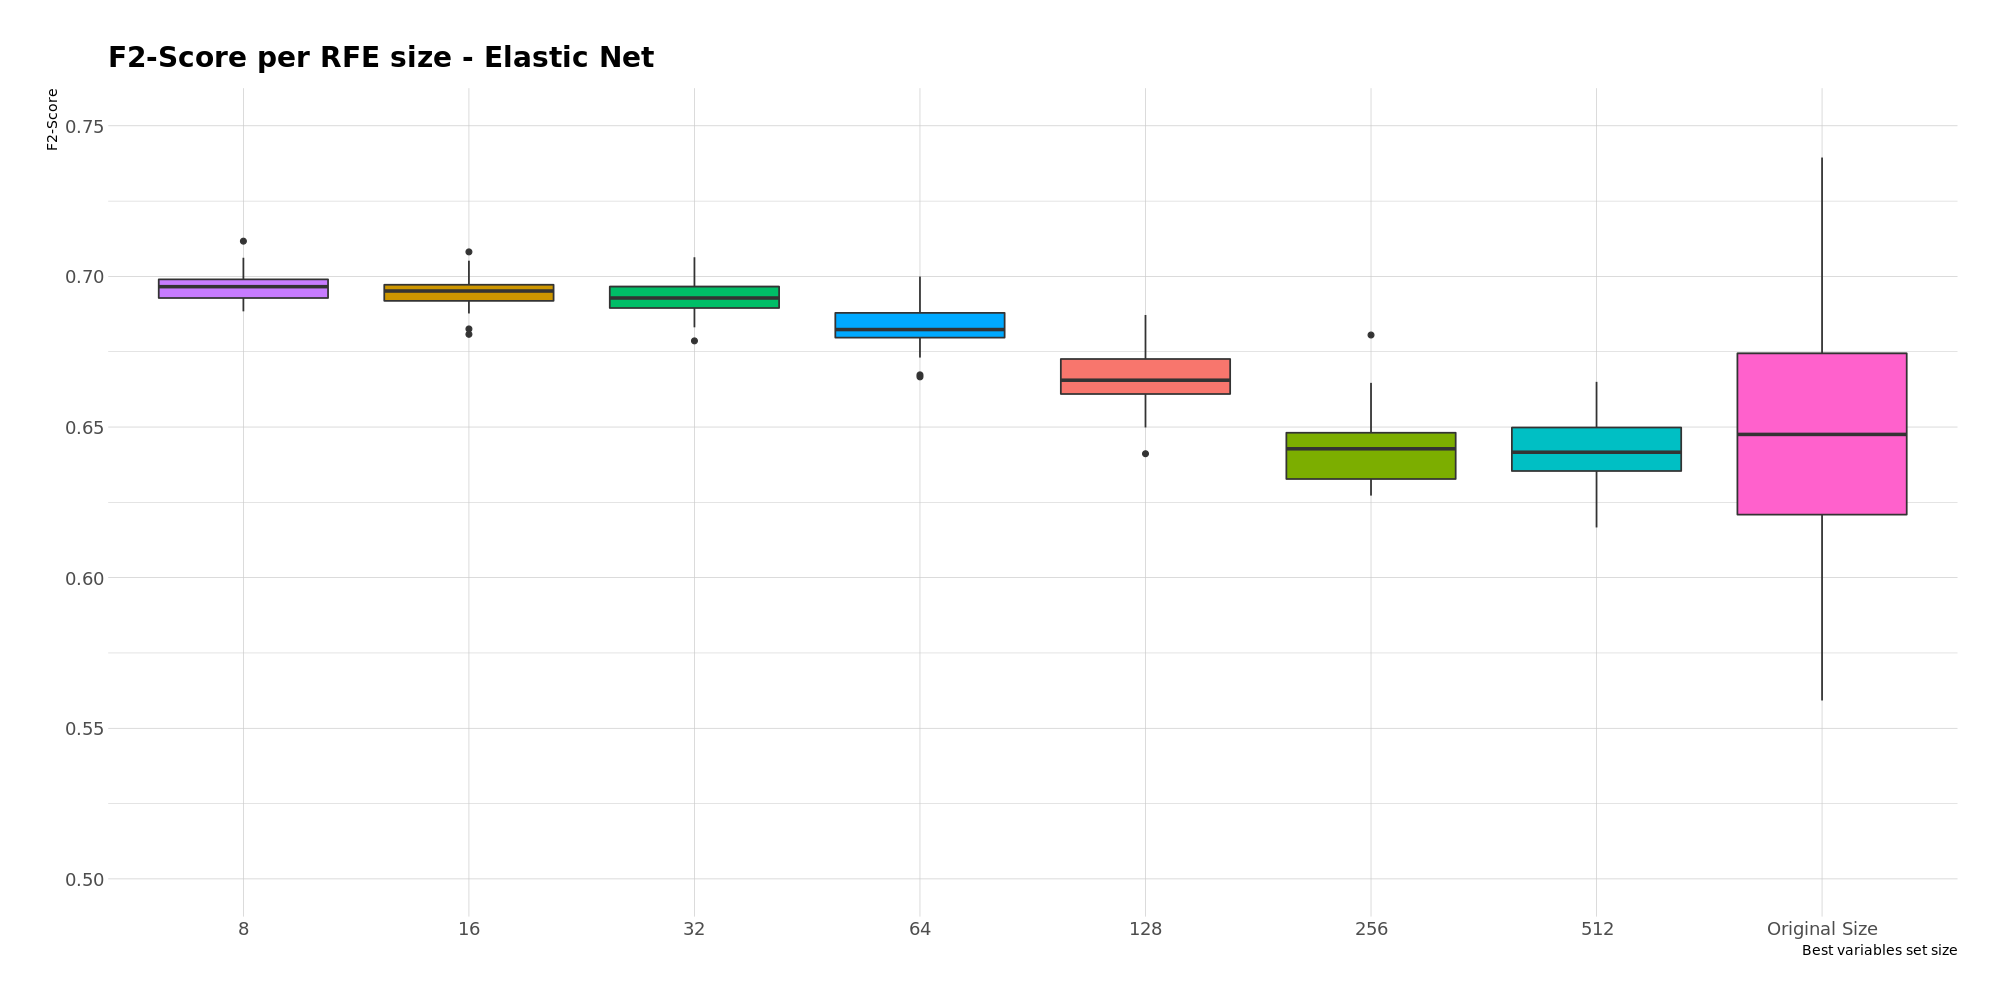
\includegraphics[scale=.21]{../reports/results/models_and_evals/summary/rfe_glmnet.png}}
    \label{fig:rfe-glmnet}
\end{figure}

\begin{figure}[H]
    \caption{Recursive feature elimination performance for Multilayer Perceptron}
    \centerline{\includegraphics[scale=.21]{../reports/results/models_and_evals/summary/rfe_mlpML.png}}
    \label{fig:rfe-mlp}
\end{figure}

\begin{figure}[H]
    \caption{Recursive feature elimination performance for Random Forest}
    \centerline{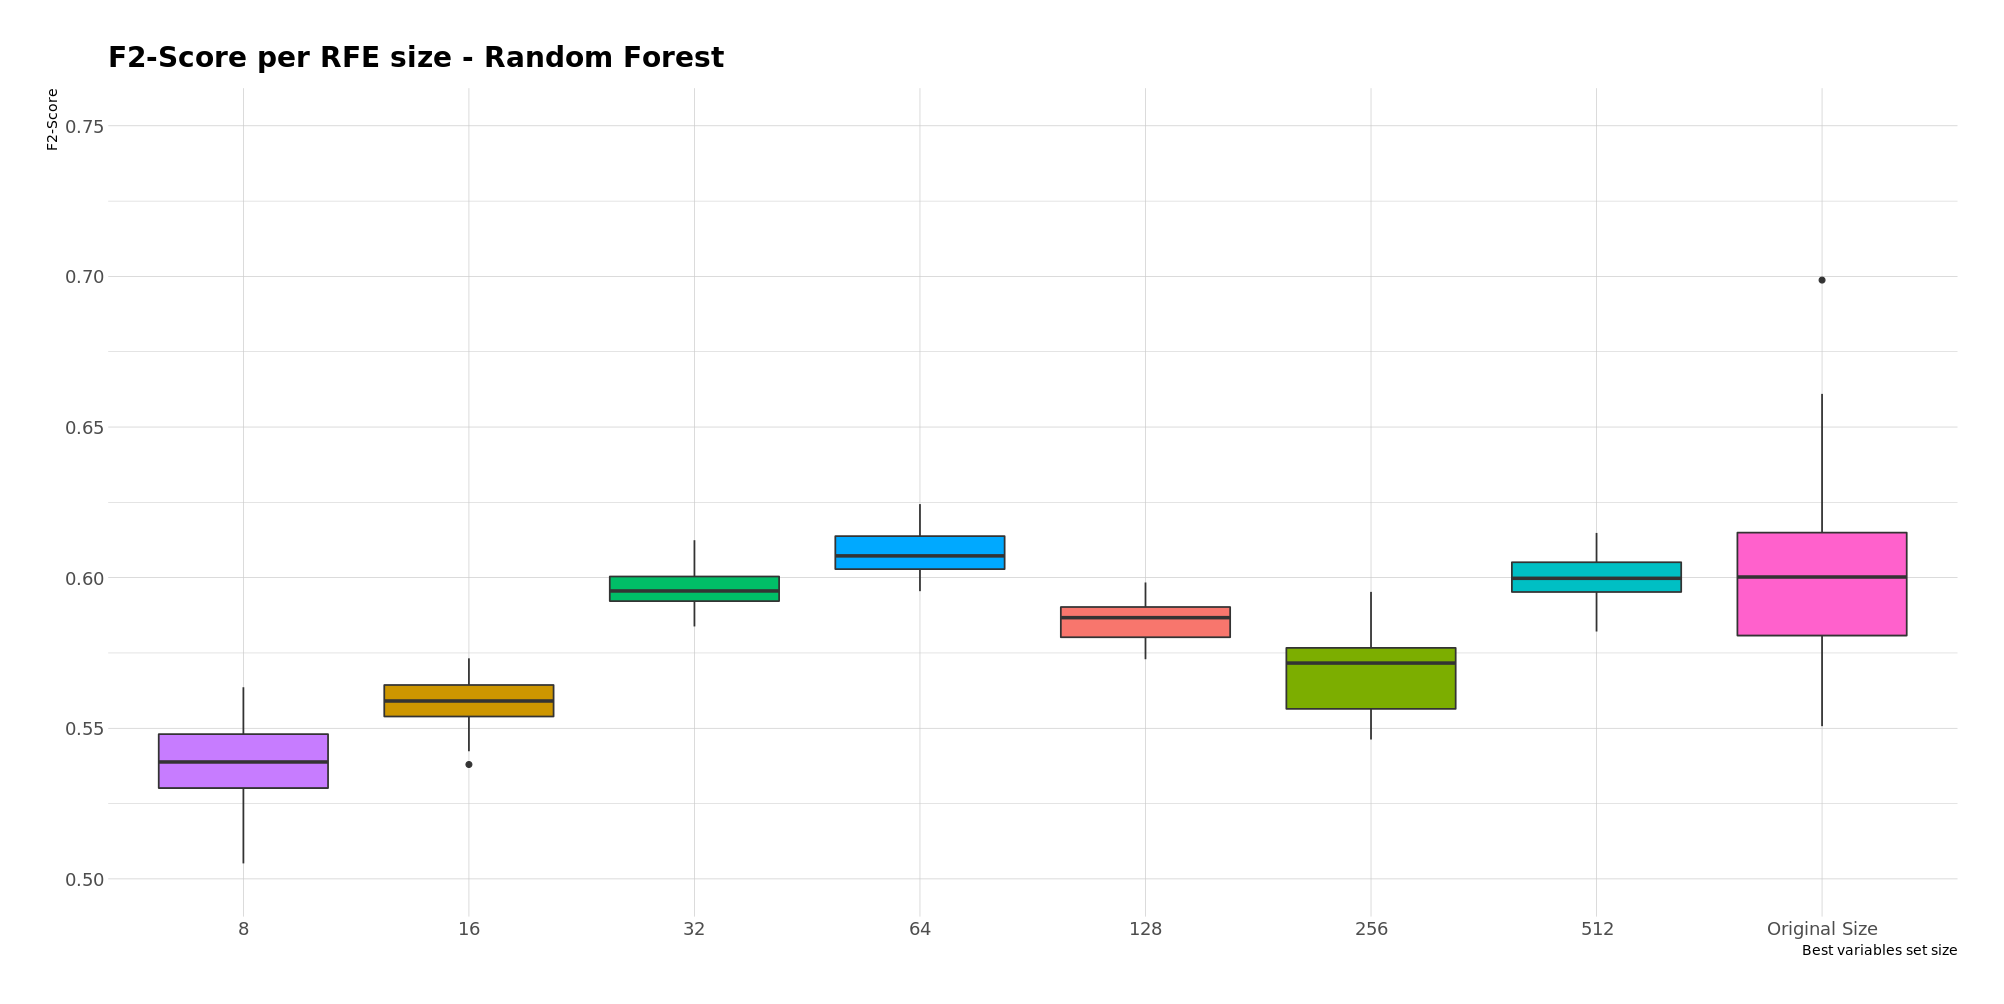
\includegraphics[scale=.21]{../reports/results/models_and_evals/summary/rfe_ranger.png}}
    \label{fig:rfe-ranger}
\end{figure}

To analyse the rankings of features importances for each algorithm, we produced "rank matrices" that can be plotted as heatmaps shown in Figures ~\ref{fig:heatmap-glmnet},~\ref{fig:heatmap-mlp}, and ~\ref{fig:heatmap-ranger}.
The idea of this visualization approach is the following: each predictor (in the vertical axis, ordered alphabetically for a naive semantical clustering) has its importance mapped to each of the trained models (with a 1:1 correspondence to a CV resample) by a ranking function \textit{F\textsubscript{rank}}.
The complete list of meanings of the top-30 most relevant attributes found using each algorithm is available in Table~\ref{tab:most-important-variables}.
The value of each attribute-to-model cell is zero when the variable does not appear in the list of most important predictors of the model.
Otherwise, it is defined as follows (where \textit{A\textsubscript{m}} is the set of best attributes of a model \textit{m}, and \textit{I(a, m)} is the index of the attribute \textit{a} in \textit{A\textsubscript{m}}):

\begin{equation}
    F_{rank}(a, m) = \frac{\#A_m - I(a, m)}{\#A_m}
\end{equation}

Our attribute-rank matrices then have higher values (indicated by brighter colors in the heatmaps) for the variables that are most important, but the magnitudes are relatively decreased given a fixed rank index for models that have larger best-variables sets.
Moreover, the values of these matrices range from 0 to 1 after normalization according to the variables sets sizes.
Thus, the intuitions to be derived from the heatmap plots of these matrices are that horizontal lines show how the feature relevances vary across the collection of trained models, and clusters of horizontal lines with uniform colors indicate the importance of semantically similar attributes.

For each algorithm, we can average the \textit{F\textsubscript{rank}}s of each predictor across the multiple resamples to obtain generalized variable importances.
More precisely, we calculate what we define as \textit{G\textsubscript{imp}(a)} (the general importance of an attribute \textit{a}), based on a set of models \textit{M}, as:

\begin{equation}
    G_{imp}(a) = \sum_{n=1}^{\#M} \frac{F_{rank}(a,m)}{\#M}
\end{equation}

In Figures ~\ref{fig:heatmap-glmnet},~\ref{fig:heatmap-mlp}, ~\ref{fig:heatmap-ranger}, we displayed only the top-30 \textit{G\textsubscript{imp}} features.
We chose 30 because it matches the number of resamples in this plot, yielding a more pleasant plot aesthetic, but most importantly because it is a sufficient and efficient size for a set of best variables to be considered in our analysis, in the sense that we do not need to discuss many predictors but the ones we discuss are relevant and insightful (especially given the best attribute sizes indicated in Figures~\ref{fig:rfe-glmnet},~\ref{fig:rfe-mlp} and~\ref{fig:rfe-ranger}).

The exception of this rule is Figure~\ref{fig:heatmap-mlp}, where only 17 features are shown.
We note that, for this algorithm, there are also relatively clearer horizontal and vertical patterns in the heatmap, and also low variance in its RFE plot (Figure~\ref{fig:rfe-mlp}).
This indicates that these models are more concise, and also homogeneous between each other.

\begin{figure}[H]
    \caption{Heatmap of attribute relevance for Elastic Net}
    \centerline{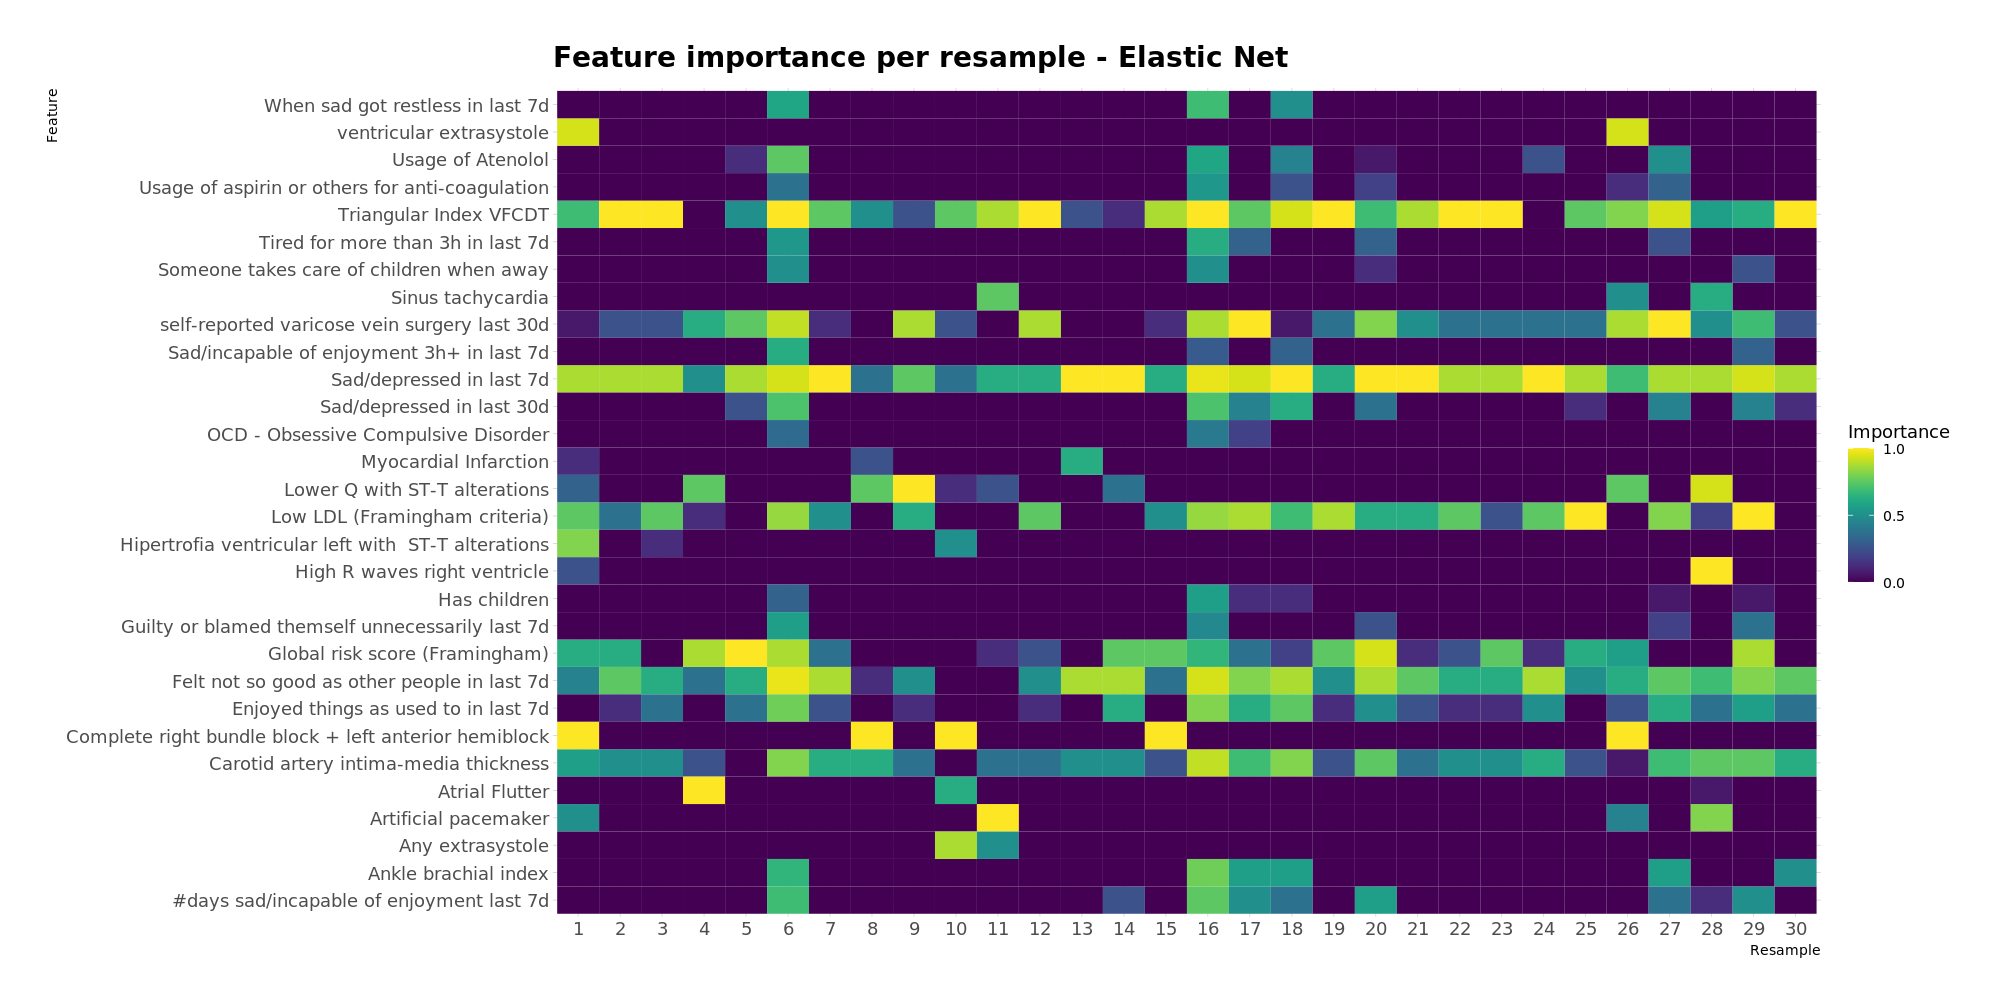
\includegraphics[scale=.21]{../reports/results/models_and_evals/summary/var_imp_resample_glmnet.png}}
    \label{fig:heatmap-glmnet}
\end{figure}

\begin{table}[H]
    \renewcommand{\arraystretch}{0.65} % Default value: 1
    \caption{Variables ranked as most important for trained models in alphabetical order}
    \begin{center}
        \begin{tabular}{l|l}
            \textit{Attribute}                & \textit{Description}                                  \\
            \hline
            \hline
            bp\_derivedA\_RAZAOPAS            & Ankle brachial index                                  \\
            cisab5                            & Tired for more than 3h in last 7d (B5)                \\
            cisae7                            & Argument fight in last 7d (E7)                        \\
            cisag1                            & Sad/depressed in last 30d (G1)                        \\
            cisag2                            & Enjoyed things as used to in last 30d (G2)            \\
            cisag4                            & Sad/depressed in last 7d (G4)                         \\
            cisag5                            & Enjoyed things as used to in last 7d (G5)             \\
            cisag6                            & \#days sad/incapable of enjoyment last 7d (G6)        \\
            cisag7                            & Sad/incapable of enjoyment 3h+ in last 7d (G7)        \\
            cisah1                            & Worst time of day for sadness last 7d (H1)            \\
            cisah2                            & Sexual desire in last 30d (H2)                        \\
            cisah3a                           & When sad, got restless in last 7d (H3a)               \\
            cisah3b                           & When sad, did things more slowly in last 7d (H3b)     \\
            cisah3c                           & When sad got less talkative in last 7d (H3c)          \\
            cisah4                            & Guilty or blamed themself unnecessarily last 7d (H4)  \\
            cisah5                            & Felt not so good as other people in last 7d (H5)      \\
            cisai8                            & How unpleasant was the worrying in last 7d (I8)       \\
            cisaj8                            & How unpleasant was the general anxiety last 7d (J8)   \\
            cisan1                            & Unpleasant thoughts kept appearing last 30d (N1)      \\
            cisao1                            & Feelings precluded things last 7d (O1)                \\
            cisao1a                           & Feelings precluded more than once last 7d (O1a)       \\
            derived\_A\_FRAMINGHAM\_CHD\_LDL  & Low LDL (Framingham criteria)                         \\
            derived\_A\_GLOBAL\_RISK          & Global risk score (Framingham)                        \\
            derived\_A\_RCPCIRVARIZESULT30D   & Self-reported varicose vein surgery in last 30d       \\
            derived\_A\_VIFA30\_PMCAT         & Familial income                                       \\
            derived\_cogA\_FLUENCIA\_LETRAF   & Fluency score with words with the letter F            \\
            derived\_nle                      & Any negative life event                               \\
            derived\_usga1                    & Carotid artery intima-media thickness                 \\
            EKG\_a\_ecgmc\_bcrd\_hae          & Complete right bundle block + left anterior hemiblock \\
            EKG\_a\_ecgmc\_esv                & ventricular extrasystole                              \\
            EKG\_a\_ecgmc\_fluttera           & Atrial Flutter                                        \\
            EKG\_a\_ecgmc\_hve\_stt           & Left ventricular hypertrophy with ST-T alterations    \\
            EKG\_a\_ecgmc\_im                 & Myocardial Infarction                                 \\
            EKG\_a\_ecgmc\_mp                 & Artificial pacemaker                                  \\
            EKG\_a\_ecgmc\_qmenor\_stt        & Lower Q with ST-T alterations                         \\
            EKG\_a\_ecgmc\_qualquer\_ex\_vent & Any extrasystole                                      \\
            EKG\_a\_ecgmc\_rvd                & High R waves right ventricle                          \\
            EKG\_a\_ecgmc\_ts                 & Sinus tachycardia                                     \\
            EKG\_a\_vfccl\_triangindex\_dt    & Triangular Index VFCDT                                \\
            home\_info\_vifa11                & Children (Q11)                                        \\
            meds\_atenolol                    & Usage of Atenolol                                     \\
            mentalvar\_\_TAG                  & GAD - Generalized Anxiety Disorder                    \\
            mentalvar\_\_TOC                  & OCD - Obsessive Compulsive Disorder                   \\
            mentalvar\_A\_SINTDEP             & Depression symptoms                                   \\
            mentalvar\_A\_SINTMEMORIA         & Concentration symptoms                                \\
            metadata\_ecga2                   & V4 value                                              \\
            negativelifeevents\_evea12        & Severe financial difficulties in last 12m (Q12)       \\
            neighborhood\_viza06              & Physical activities conditions in neighbourhood (Q6)  \\
            others\_cssa3                     & Usage of aspirin or others for anti-coagulation       \\
            others\_esca03                    & Work-related self-evaluation (Q3)                     \\
            social\_support\_capa57           & Someone takes care of children when away (Q57)        \\
            \hline
        \end{tabular}
    \end{center}
    \label{tab:most-important-variables}
\end{table}

\begin{figure}[H]
    \caption{Heatmap of attribute relevance for Multilayer Perceptron}
    \centerline{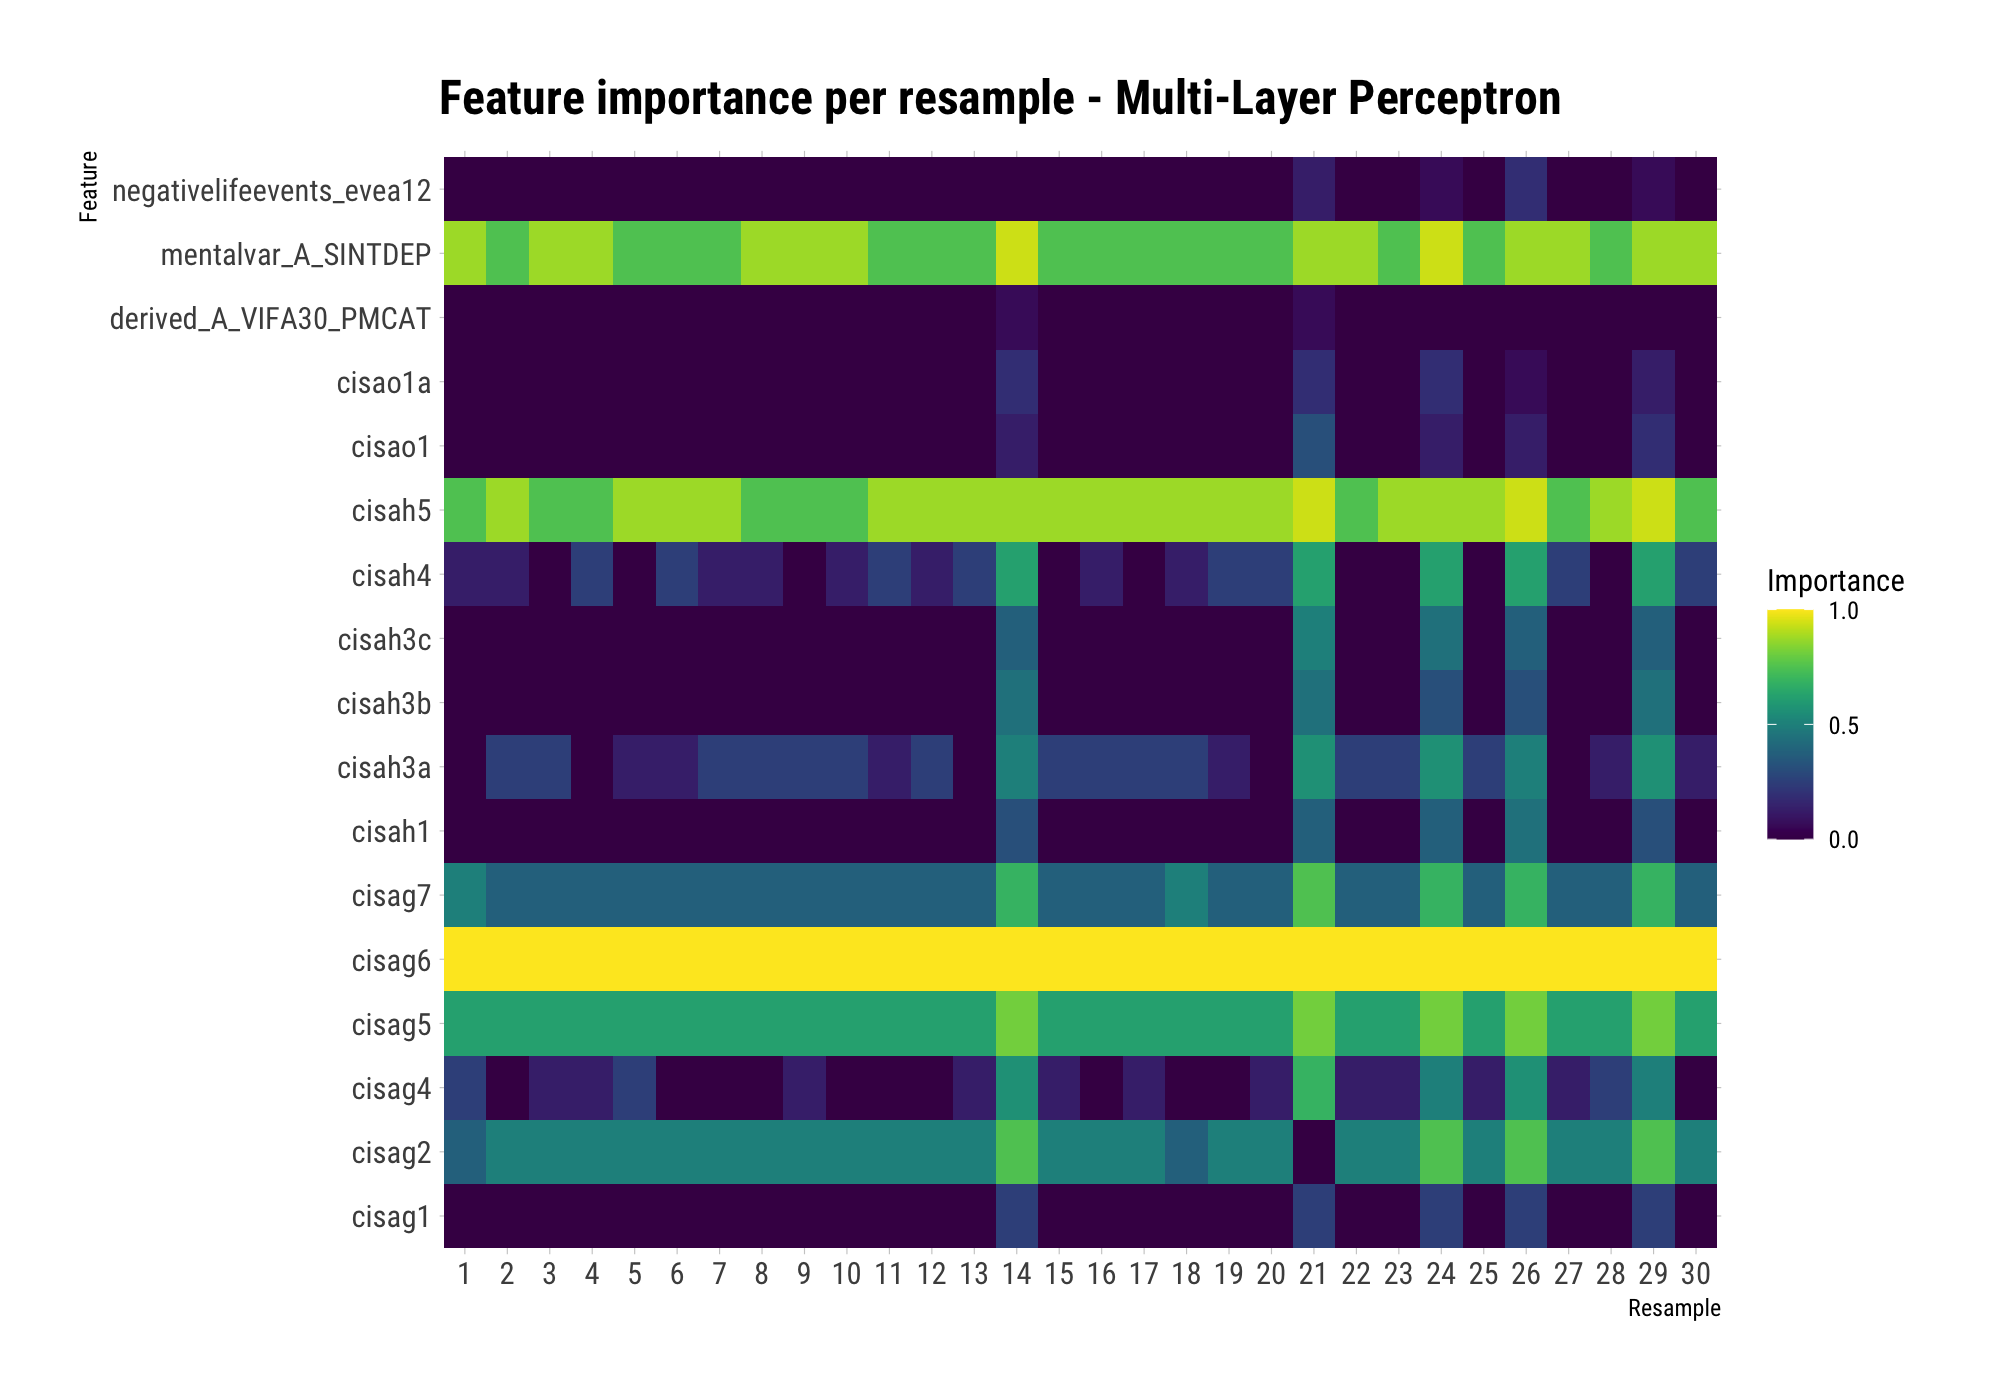
\includegraphics[scale=.21]{../reports/results/models_and_evals/summary/var_imp_resample_mlpML.png}}
    \label{fig:heatmap-mlp}
\end{figure}

\begin{figure}[H]
    \caption{Heatmap of attribute relevance for Random Forest}
    \centerline{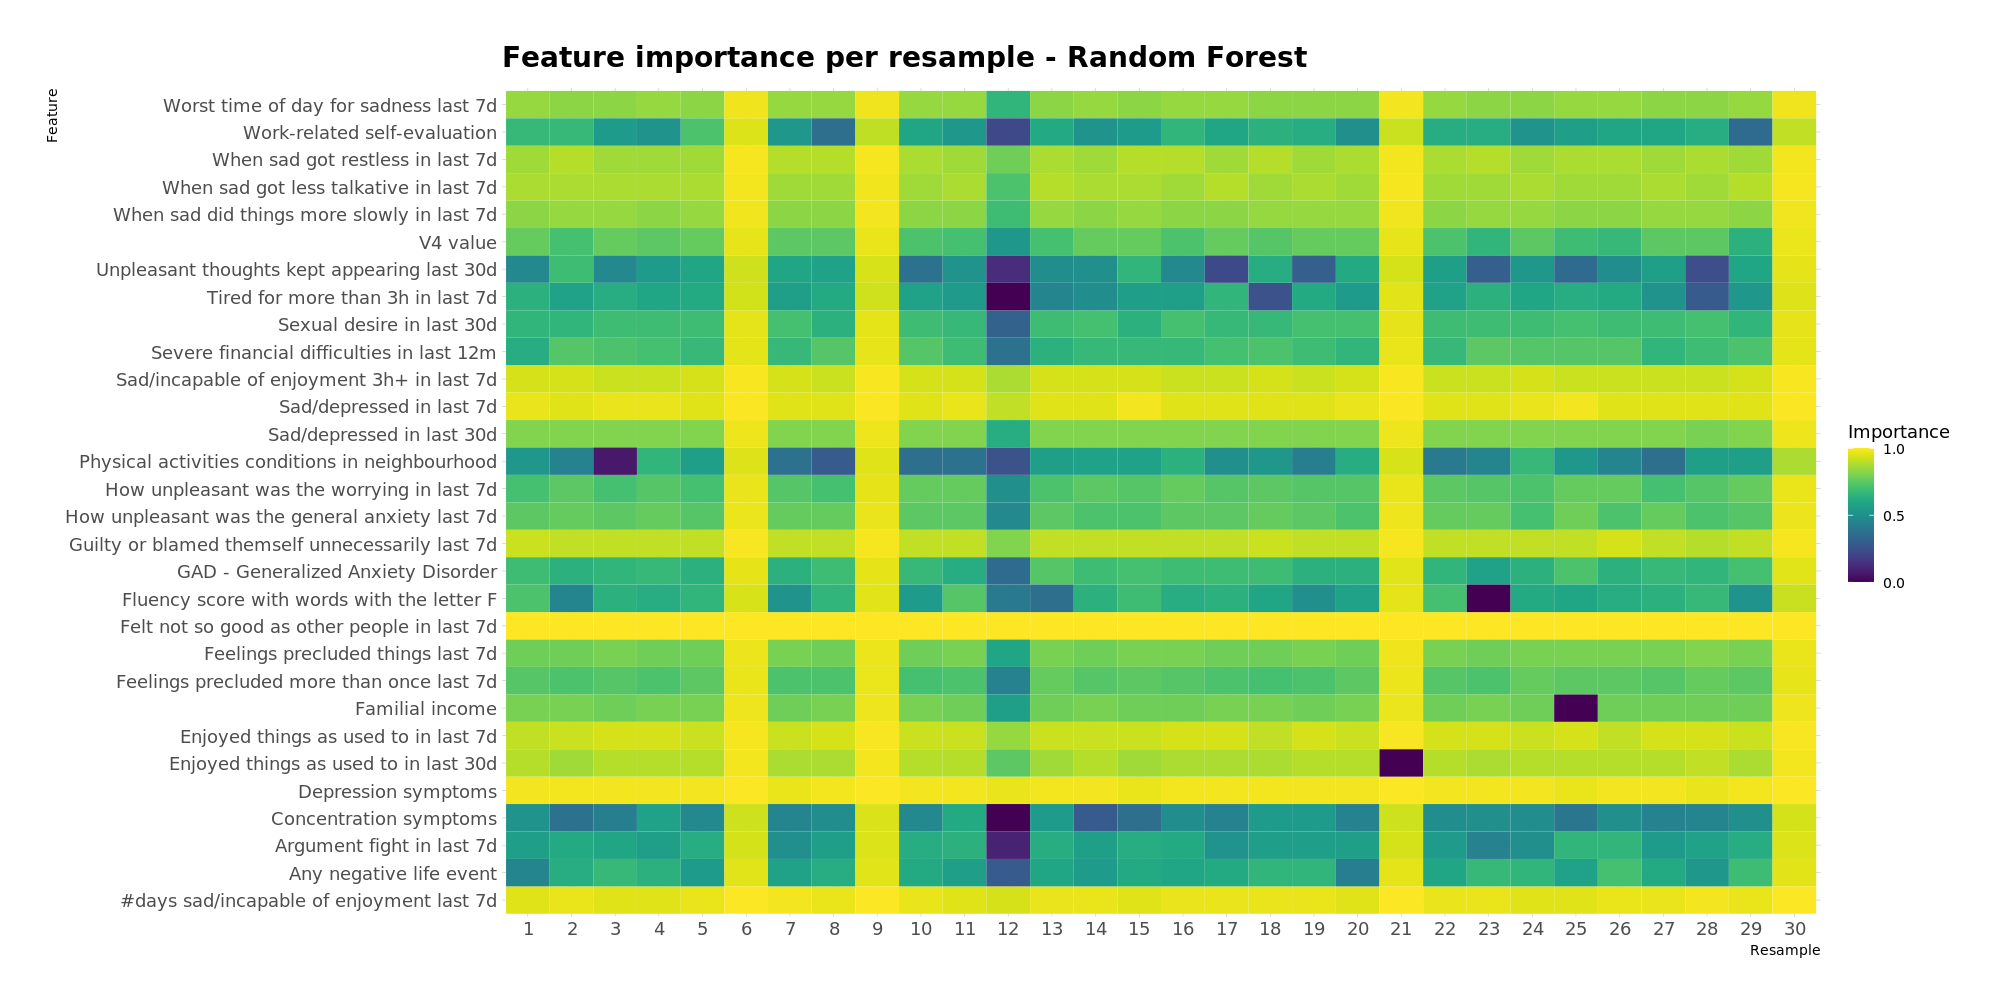
\includegraphics[scale=.21]{../reports/results/models_and_evals/summary/var_imp_resample_ranger.png}}
    \label{fig:heatmap-ranger}
\end{figure}

\pagebreak

Another useful employment of our \textit{G\textsubscript{imp}} metric is to arrange the variables according to it, ordered from highest to lowest, so that we can understand at a glance what each algorithm tends to consider most when predicting the classes of instances.
This is shown in Figures~\ref{fig:rank-glmnet},~\ref{fig:rank-mlp}, and~\ref{fig:rank-ranger}.

In diametrical opposition to the MLPs' simplicity, RFs learned that many more predictors are relevant for correct classification.
This is indicated by the already described performance peak at 64 RFE variables, by the \textit{F\textsubscript{rank}} heatmap (Figure ~\ref{fig:heatmap-ranger}) being overall brighter than the MLP's and EN's heatmaps, and by the top 30 attributes having small \textit{G\textsubscript{imp}} differences between each other (Figure ~\ref{fig:rank-ranger}).

On the other hand, based on the features heatmap and the rank plot of Figures~\ref{fig:heatmap-glmnet} and~\ref{fig:rank-glmnet}, we can place the elastic nets in an "intermediate" spot between the MLPs and the RFs regarding simplicity and homogeneity.
Figure~\ref{fig:heatmap-glmnet} indicates patterns of some features being considered relevant across different resamples, but the patterns are not so clear and uniform as the MLP's, and the variables are not so numerous or few as the RF's or MLP's, respectively.

\begin{figure}[H]
    \caption{Rank attribute relevance for Elastic Net}
    \centerline{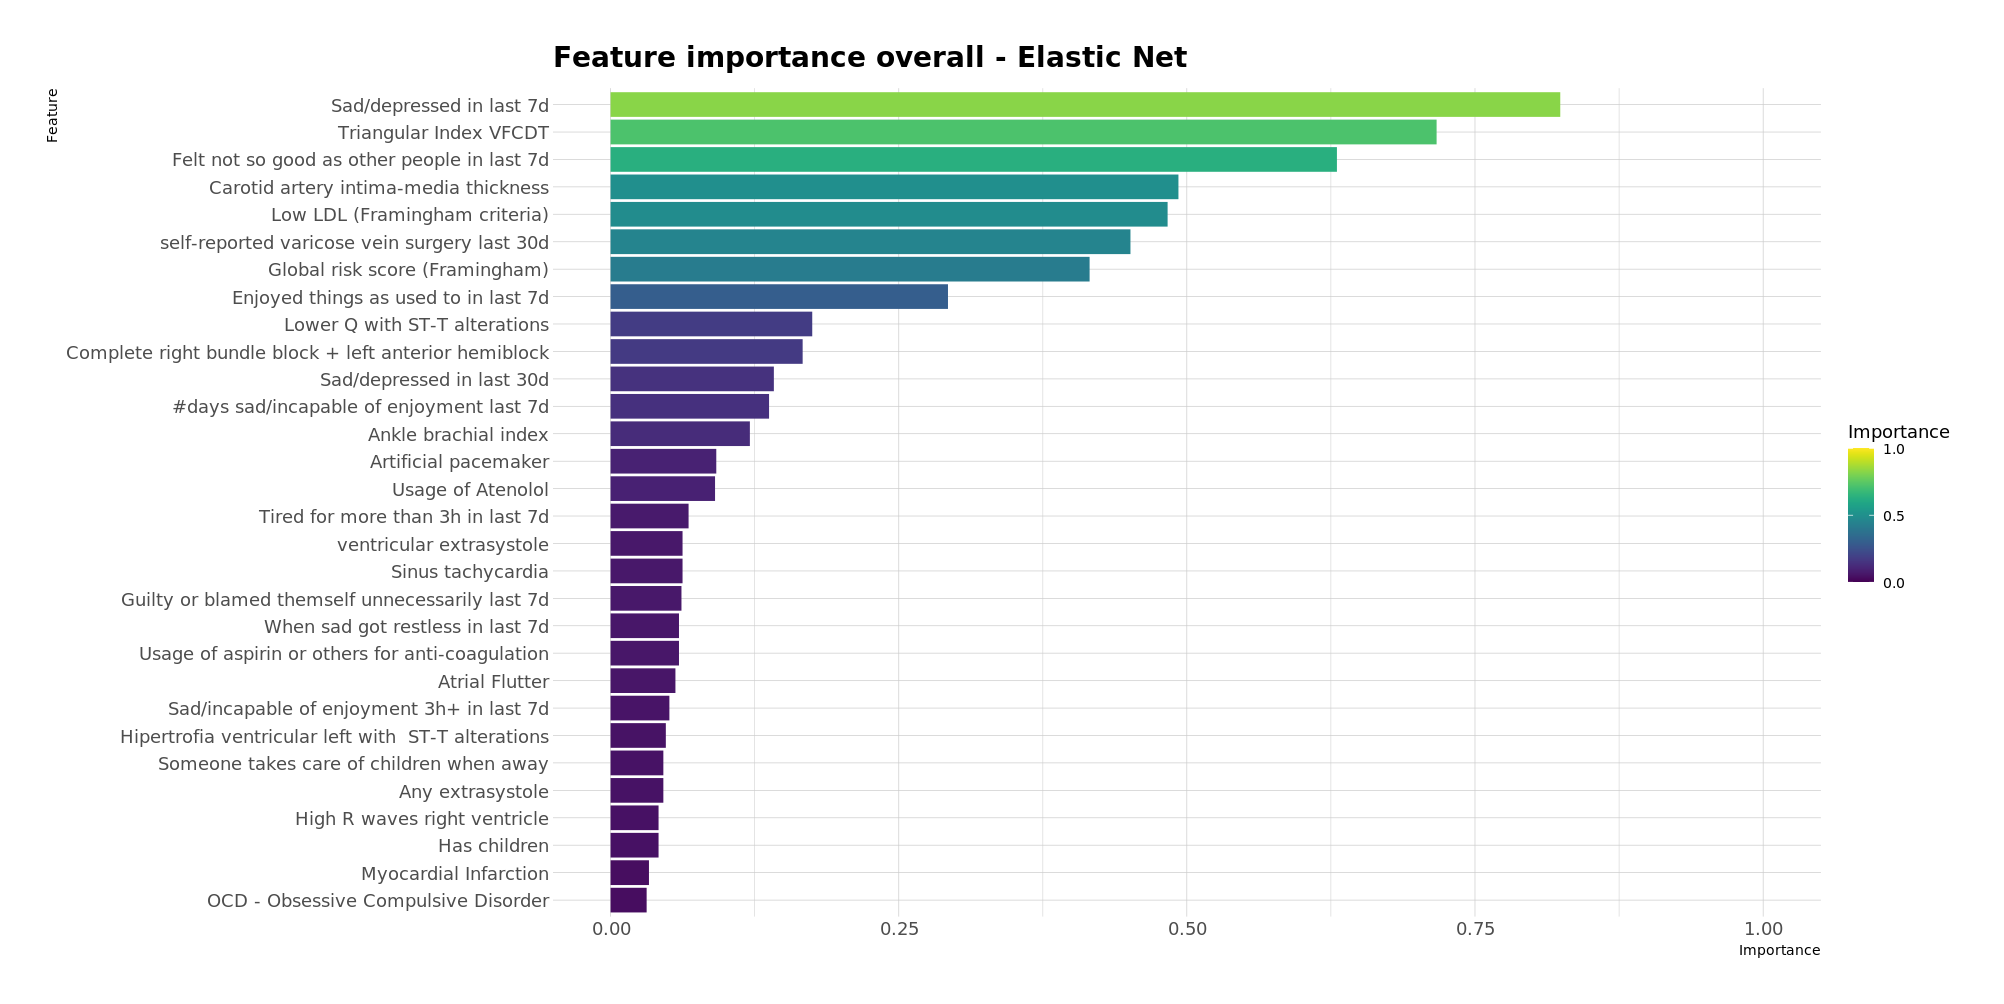
\includegraphics[scale=.21]{../reports/results/models_and_evals/summary/var_imp_glmnet.png}}
    \label{fig:rank-glmnet}
\end{figure}

\begin{figure}[H]
    \caption{Rank of attribute relevance for Multilayer Perceptron}
    \centerline{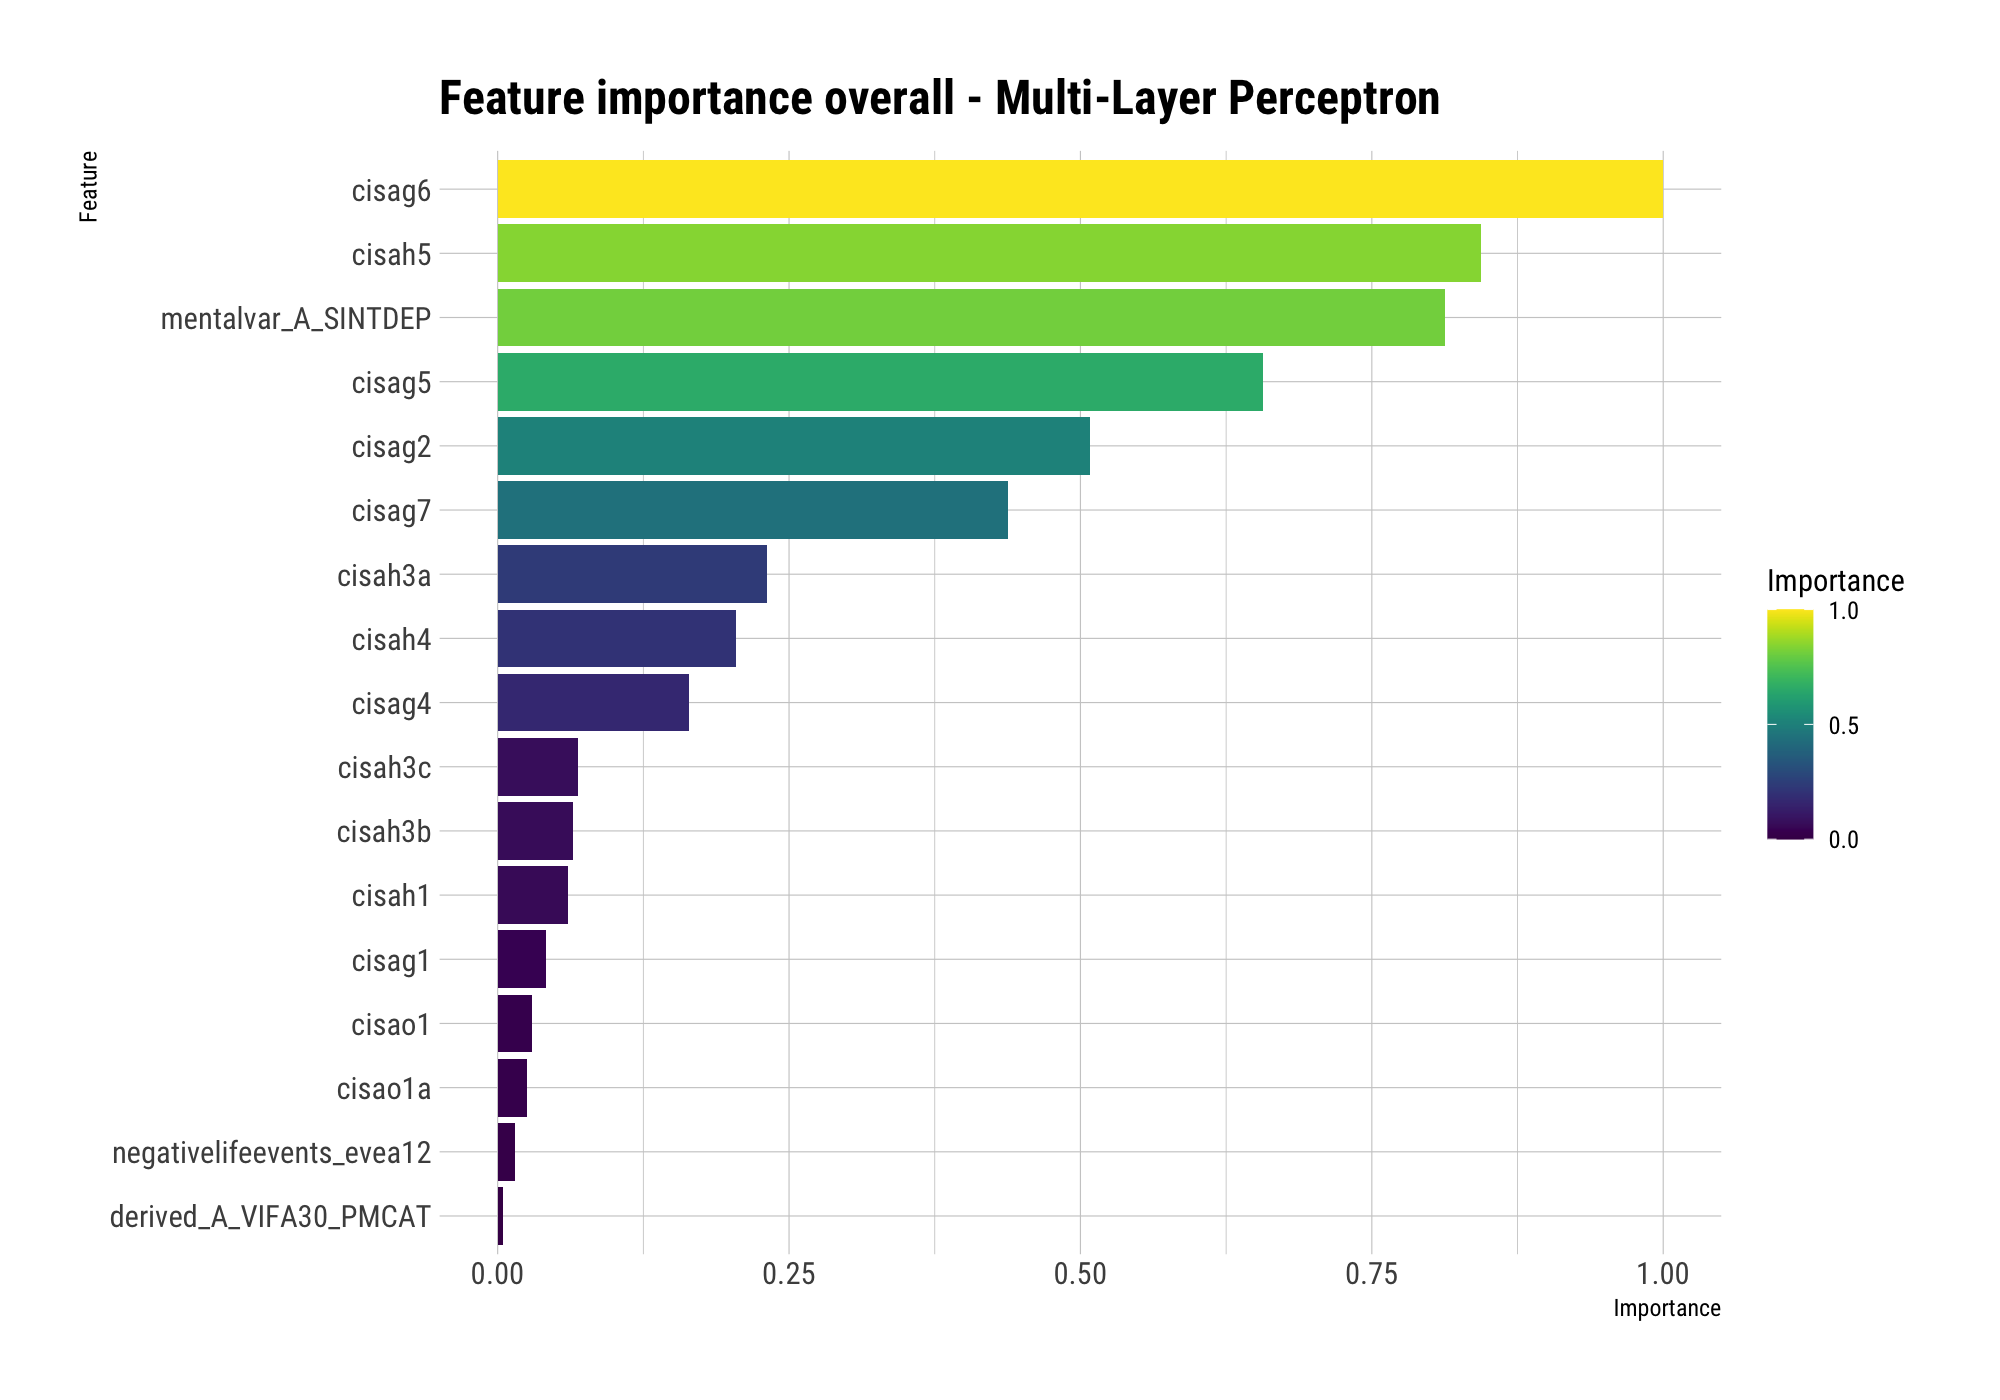
\includegraphics[scale=.21]{../reports/results/models_and_evals/summary/var_imp_mlpML.png}}
    \label{fig:rank-mlp}
\end{figure}

\begin{figure}[H]
    \caption{Rank of attribute relevance for Random Forest}
    \centerline{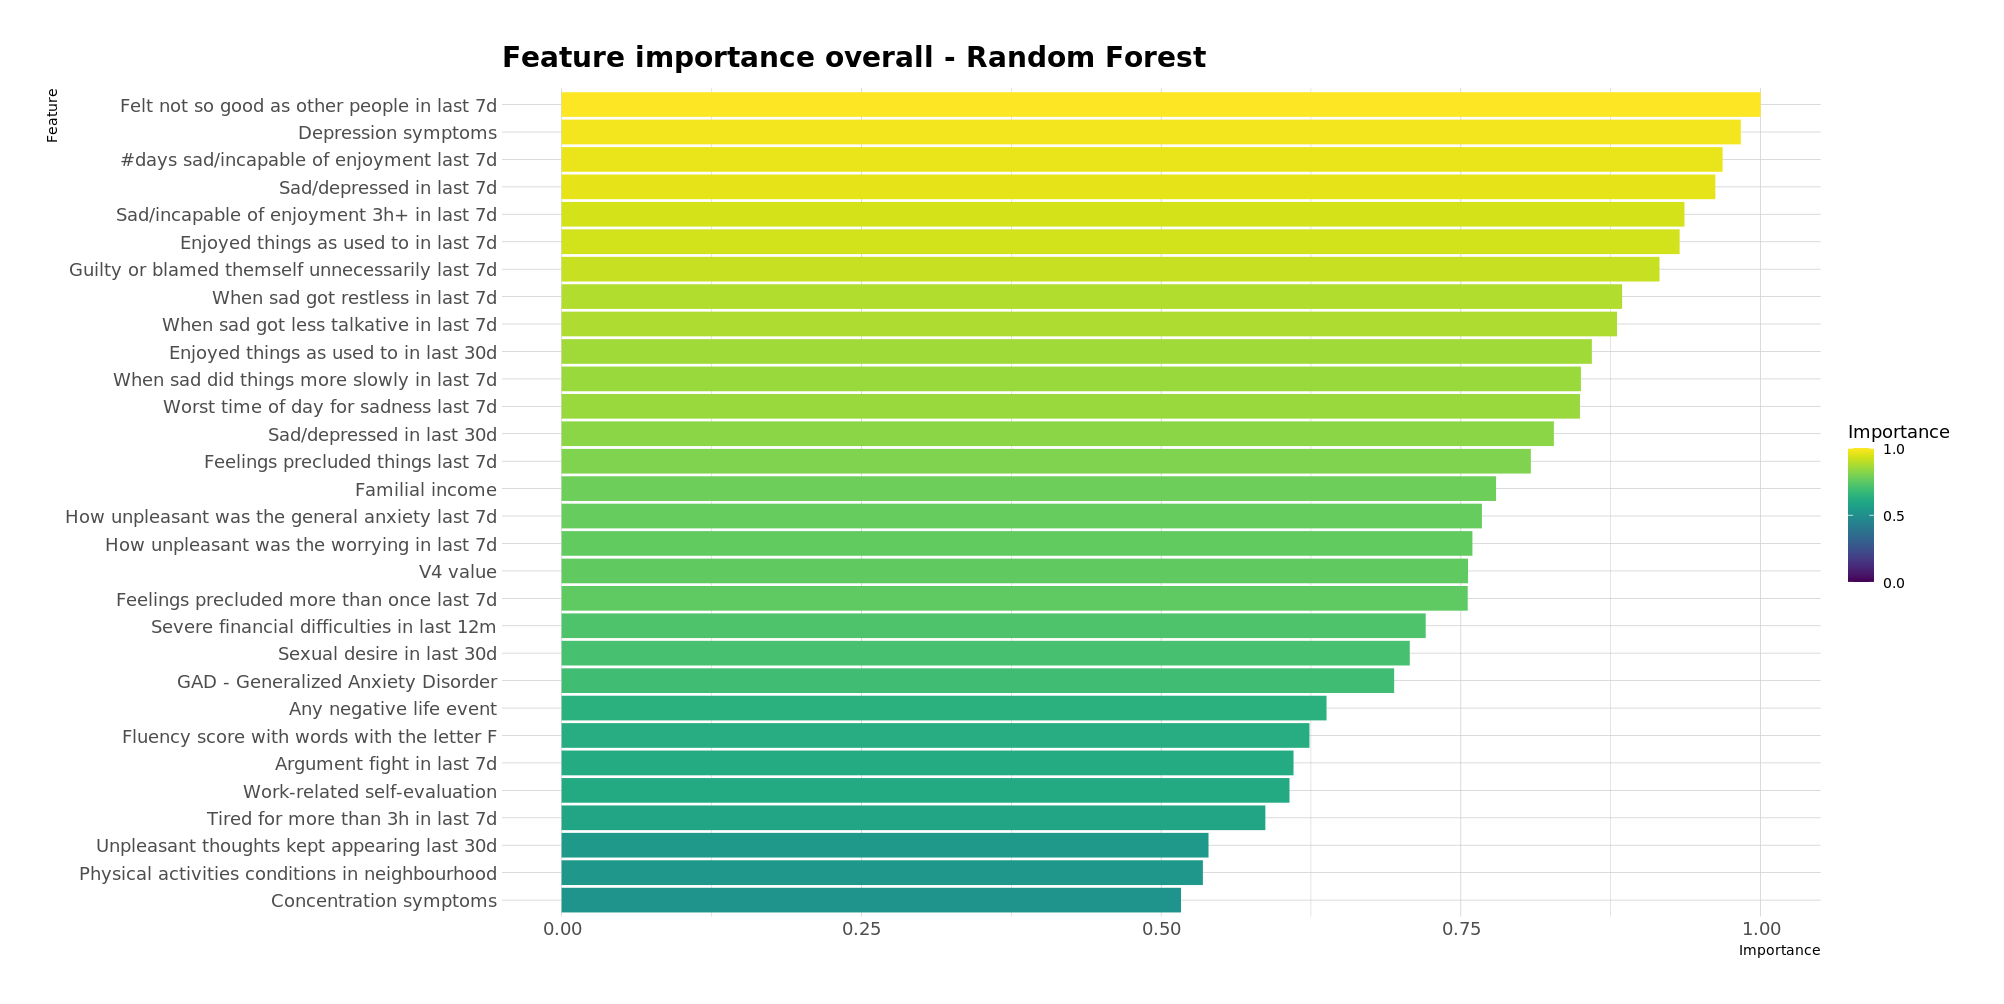
\includegraphics[scale=.21]{../reports/results/models_and_evals/summary/var_imp_ranger.png}}
    \label{fig:rank-ranger}
\end{figure}

\pagebreak

The combination of the three \textit{F\textsubscript{rank}} matrices (which, despite what is shown in Figures~\ref{fig:heatmap-glmnet},~\ref{fig:heatmap-mlp}, ~\ref{fig:heatmap-ranger}, and~\ref{fig:heatmap-ensemble}, includes \textit{all} predictors in the dataset) by averaging the values of the cells in matching positions gives us a form of condensed and summarized knowledge on the criteria used by our classifiers and roughly estimates the attribute importances of our class-probability-averaging ensemble.
We then calculate each predictor's \textit{G\textsubscript{imp}} to sort them by this quantity and again plot the top 30 in a heatmap and in a column chart as was done with the single classifiers.

\begin{figure}[H]
    \caption{Heatmap of attribute relevance for Averaging Ensemble}
    \centerline{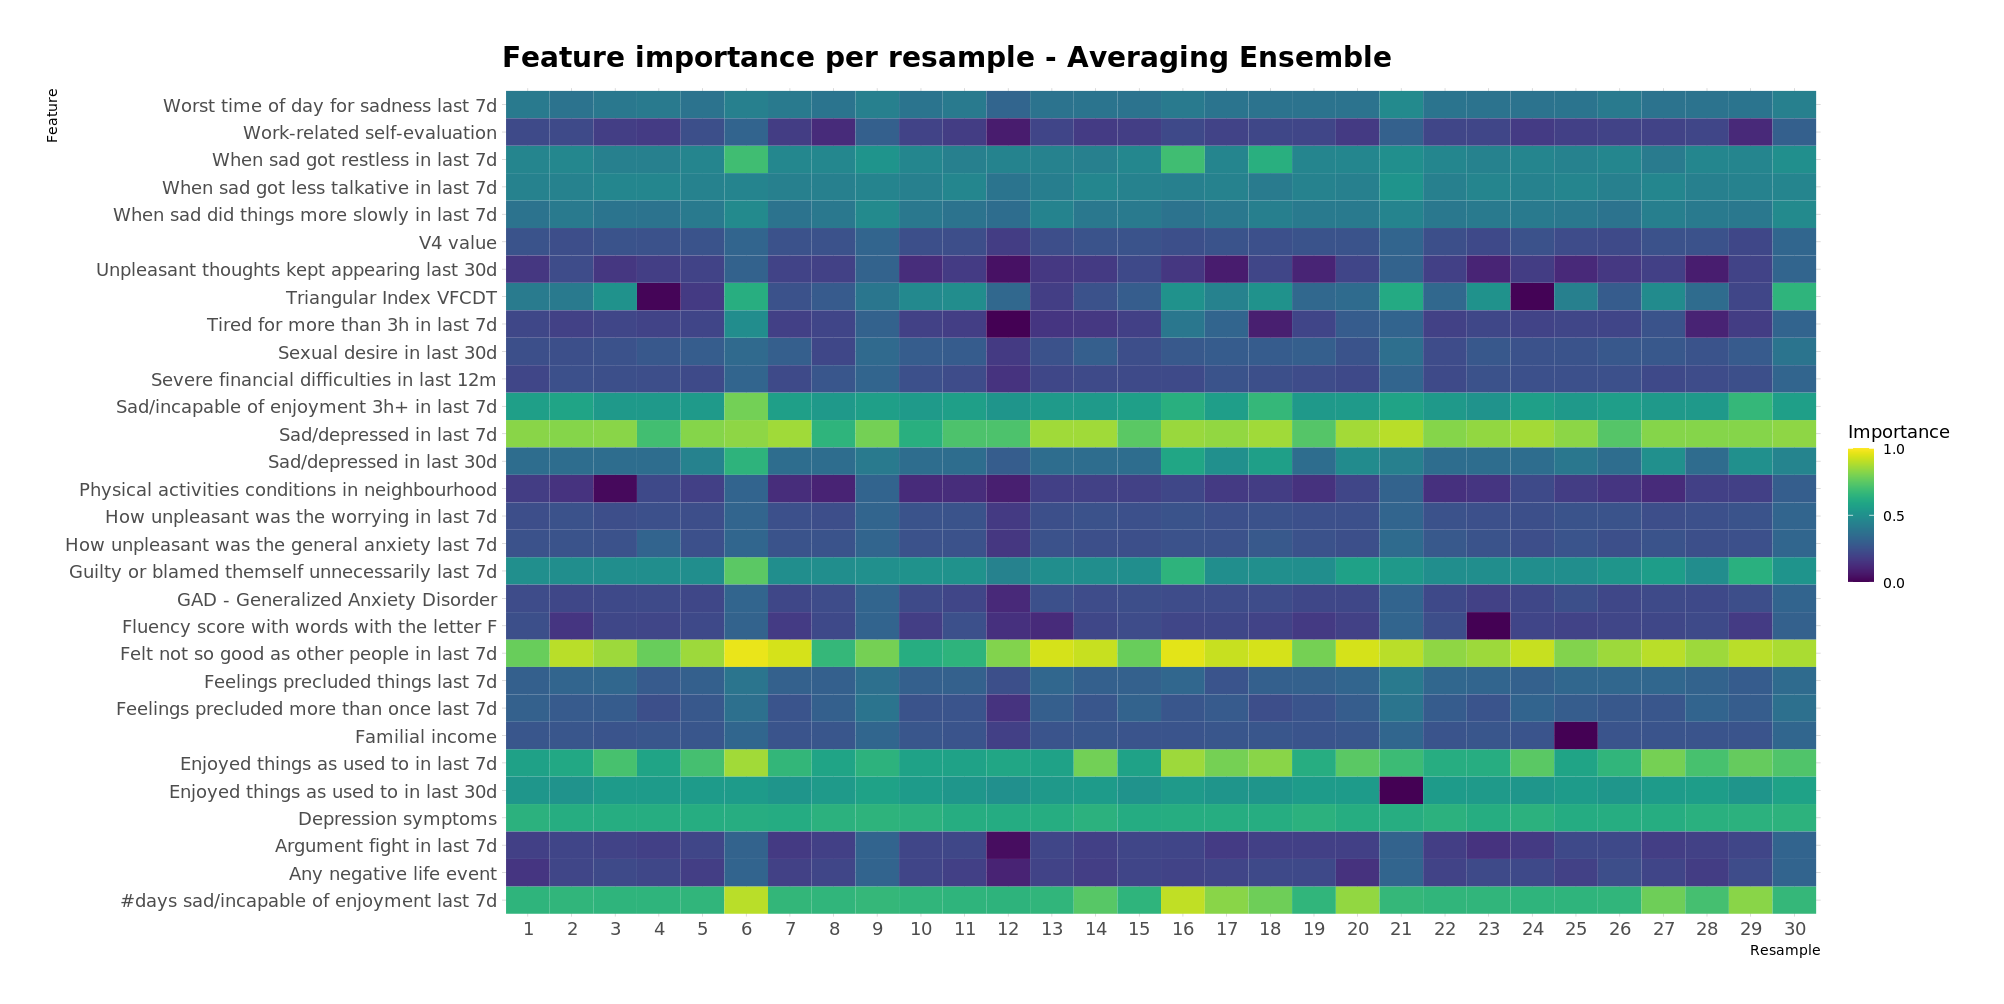
\includegraphics[scale=.22]{../reports/results/models_and_evals/summary/var_imp_resample_aggregation.png}}
    \label{fig:heatmap-ensemble}
\end{figure}

\begin{figure}[H]
    \caption{Rank of attribute relevance for Averaging Ensemble}
    \centerline{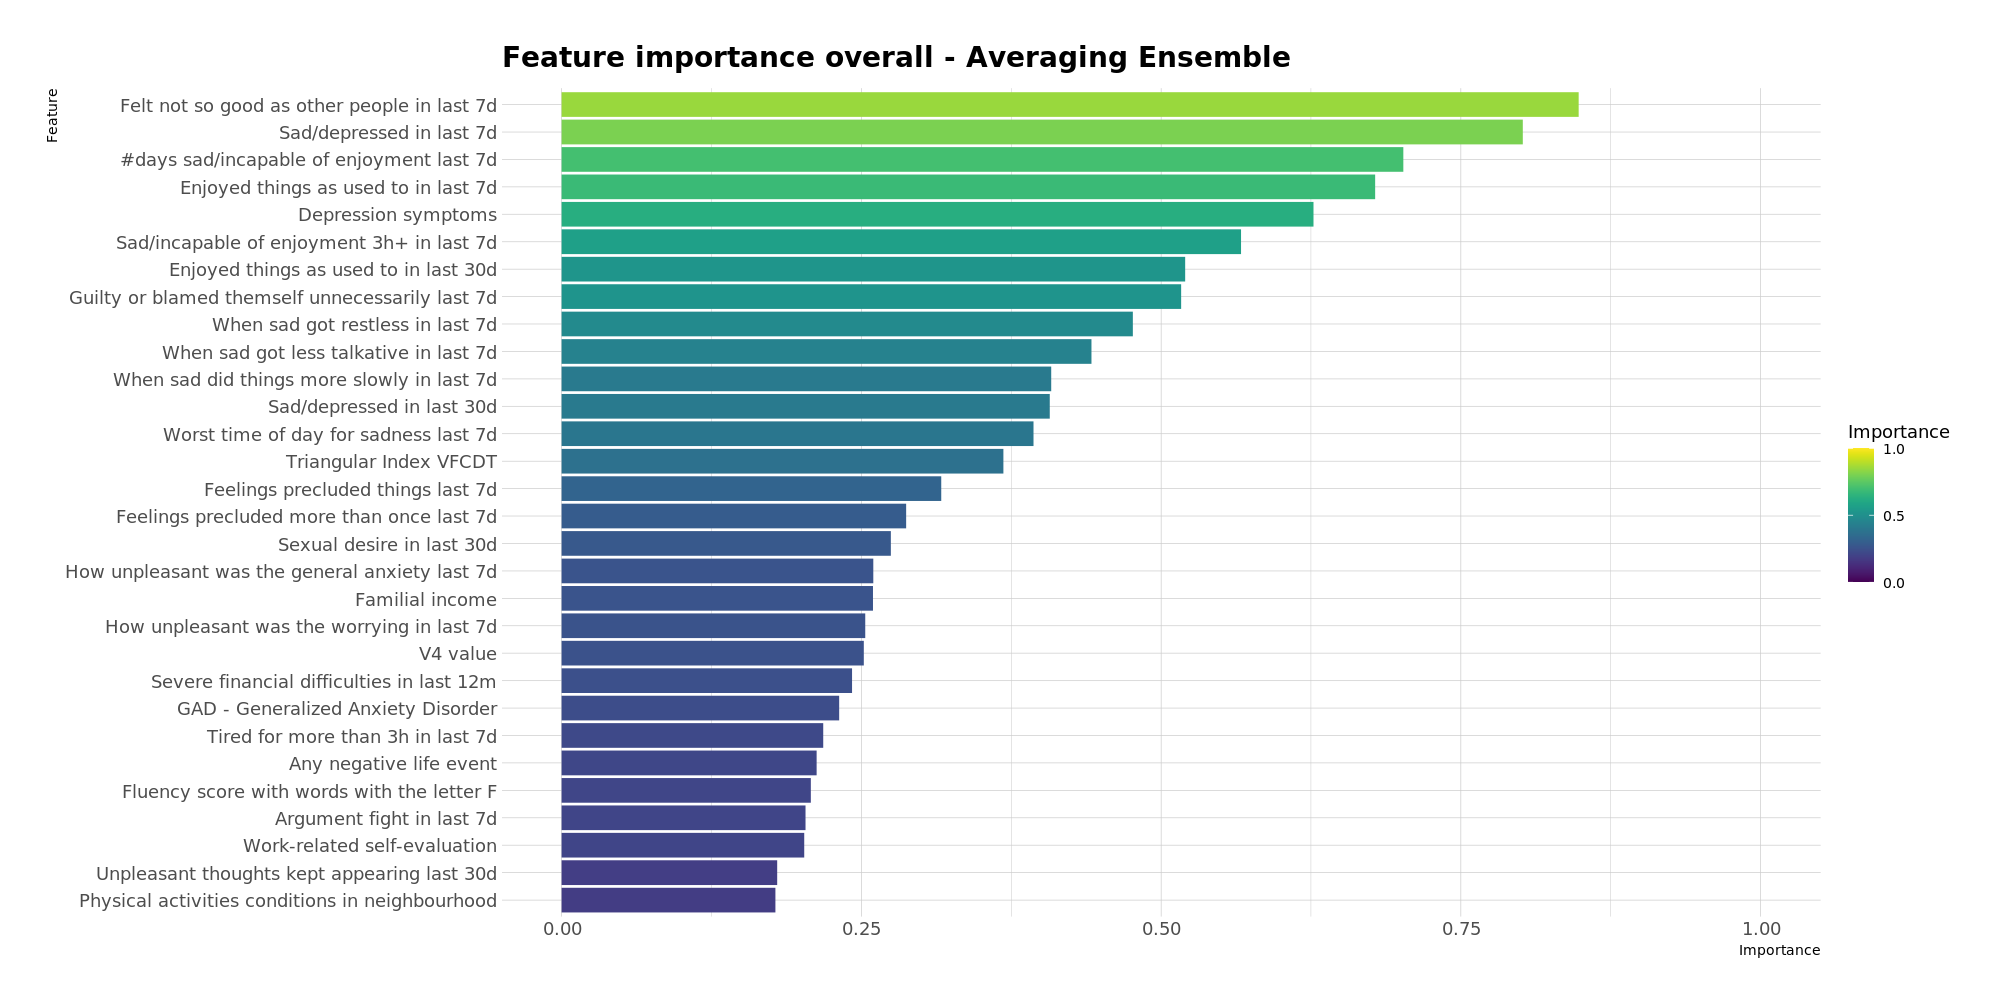
\includegraphics[scale=.21]{../reports/results/models_and_evals/summary/var_imp_aggregation.png}}
    \label{fig:rank-ensemble}
\end{figure}

Regarding the chosen variables per se, Figure~\ref{fig:rank-ensemble} gives us a clear top 5 indicated by the brightest colors and a rather abrupt \textit{G\textsubscript{imp}} jump from the fifth to sixth position, ordered by importance: \textit{cisah5}, \textit{cisag6}, \textit{cisag4}, \textit{cisag5}, and \textit{mentalvar\_A\_SINTDEP}.
All of these are responses to the CIS-R questionnaire, from section G (depression) and H (depressive ideas), safe for \textit{mentalvar\_A\_SINTDEP}, but it relates to the same general theme.
It is worth going over the exact definition of each of the respective questions here, for the analysis and understanding of the models.
Thus, the top-5 variables are, ordered by relevance:

\begin{itemize}
    \item CIS-H5: \textit{During the past week, have you been feeling you are not as good as other people?}
    \item CIS-G6: \textit{Since last (DAY OF WEEK) on how many days have you felt sad, miserable or depressed/unable to enjoy or take an interest in things?}
    \item CIS-G4: \textit{In the past week have you had a spell of feeling sad, miserable, or depressed? Use informant's own words if possible}
    \item CIS-G5: \textit{In the past week have you been able to enjoy or take an interest in things as much as usual? Use informant's own words if possible}
\end{itemize}

\pagebreak

Question H5 stands-out from the others, for its meaning and its calculated \textit{G\textsubscript{imp}} - this indicates our models have an overall consensus that feeling inferior to other people plays a decisive role in increasing the chance of presenting suicidality.
Both G4 and G6 reveal whether the interviewee had been feeling acute sadness, and the G5 and G6 pair provide information on people's loss of interest in things, such that they are not as enjoyable as before.

In short, our models consider as most relevant to their predictions degrees of:
\begin{enumerate}
    \item \textbf{feelings of inferiority} (\textit{cisah5});
    \item \textbf{sadness} (\textit{cisag4, cisag6, cisag7});
    \item \textbf{disappearance of interests} (\textit{cisag2, cisag7});
    \item \textbf{unnecessary guilt} (\textit{cisah4});
    \item \textbf{energy (disposition)} (\textit{cisah3a, cisah3b, cisah3c, cisab5});
    \item \textbf{preclusion} of activities including chores and leisure for bad feelings (\textit{cisao1, cisao1a});
    \item \textbf{income} (\textit{derived\_A\_VIFA30\_PMCAT, negativelifeevents\_evea12});
    \item \textbf{anxiety} (\textit{cisaj8, mentalvar\_A\_TAG});
    \item \textbf{worrying} (\textit{cisai8});
    \item \textbf{libido} (\textit{cisah2});
    \item \textbf{irritability} (\textit{cisae7});
    \item \textbf{obsessions} - or at least recurring bad thoughts (\textit{cisan1});
    \item \textbf{physical activities} (\textit{neighborhood\_viza06)}.
\end{enumerate}

Some outlier variables are found, which cannot be associated with another factor without being too speculative if no further studies on this particular variable are conducted, such as \textit{derived\_cogA\_FLUENCIA\_LETRAF}.
Some predictors relate to physical characteristics and conditions (e.g. \textit{EKG\_a\_vfccl\_triangindex}) in the overall score, but they are found more prominently in the elastic nets' \textit{G\textsubscript{imp}} rank (Figure~\ref{fig:rank-glmnet}), like \textit{derived\_A\_GLOBAL\_RISK} that relate to physical activities, overweight, obesity and metabolic syndrome, and smoking ~\cite{Coke2010}.
